\documentclass[10pt, ucs, pdf,aspectratio=169]{beamer}
\usepackage[T1, T2A]{fontenc}
% Входная кодировка utf-8
\usepackage[utf8]{inputenc}
% Поддержка русского и английского. В частности переносы
\usepackage[english,russian]{babel}

% Theme for beamer presentation.
% \usepackage{beamerthemesplit}
% Other themes include: beamerthemebars, beamerthemelined,
%                       beamerthemetree, beamerthemetreebars

\usetheme{Boadilla}
% \usecolortheme{seahorse}

\newtheorem{ru_the}{Теорема}
\renewenvironment{Theorem}{\begin{ru_the}}{\end{ru_the}}
\setbeamertemplate{navigation symbols}{}

\newcommand{\inp}[1]{\input{../../out/#1}}
\newcommand{\characteristic}[2]{\inp{#1/characteristics/#2}}
\newcommand{\descriptive}[2]{\inp{#1/descriptive/#2}}
\newcommand{\test}[3]{\inp{#1/test/#2/#3}}
\newcommand{\normaldistr}{$\mathcal{N}(\descriptive{original}{mean}, \descriptive{original}{variance})$}

\logo{
\includegraphics[width=1cm,height=1cm,keepaspectratio]{Logo_BSU.jpg}}
\title[Анализ и прогнозирование гидрологических данных]{Анализ и прогнозирование гидрологических данных}    % Enter your title between curly braces
\author[Павлов Александр]{Павлов Александр Сергеевич}                 % Enter your name between curly braces
% \institute{Кафедра Теории Вероятностей и Математической Статистики}      % Enter your institute name between curly braces
\date{\today}                    % Enter the date or \today between curly braces

\begin{document}

% Creates title page of slide show using above information
\begin{frame}
  \titlepage
\end{frame}

% \section[План]{}

% % Creates table of contents slide incorporating
% % all \section and \subsection commands
% \begin{frame}
%   \tableofcontents
% \end{frame}


\section{}

\begin{frame}
  \frametitle{Постановка задачи}   % Insert frame title between curly braces

  \begin{itemize}
    \item Предварительный статистический анализ данных
    \item Исследование статистических свойств оценки вариограммы
    \item Вариограммный анализ
    \item Прогнозирование значений временного ряда методом Кригинг
  \end{itemize}
\end{frame}

\section{Обзор реализованного программного обеспечения}

\subsection{Модуль предварительного анализа}

\begin{frame}
  \frametitle{Первичный анализ и описательные статистики}   % Insert frame title between curly braces
   \begin{columns}[c]
   \column{4.5in}
  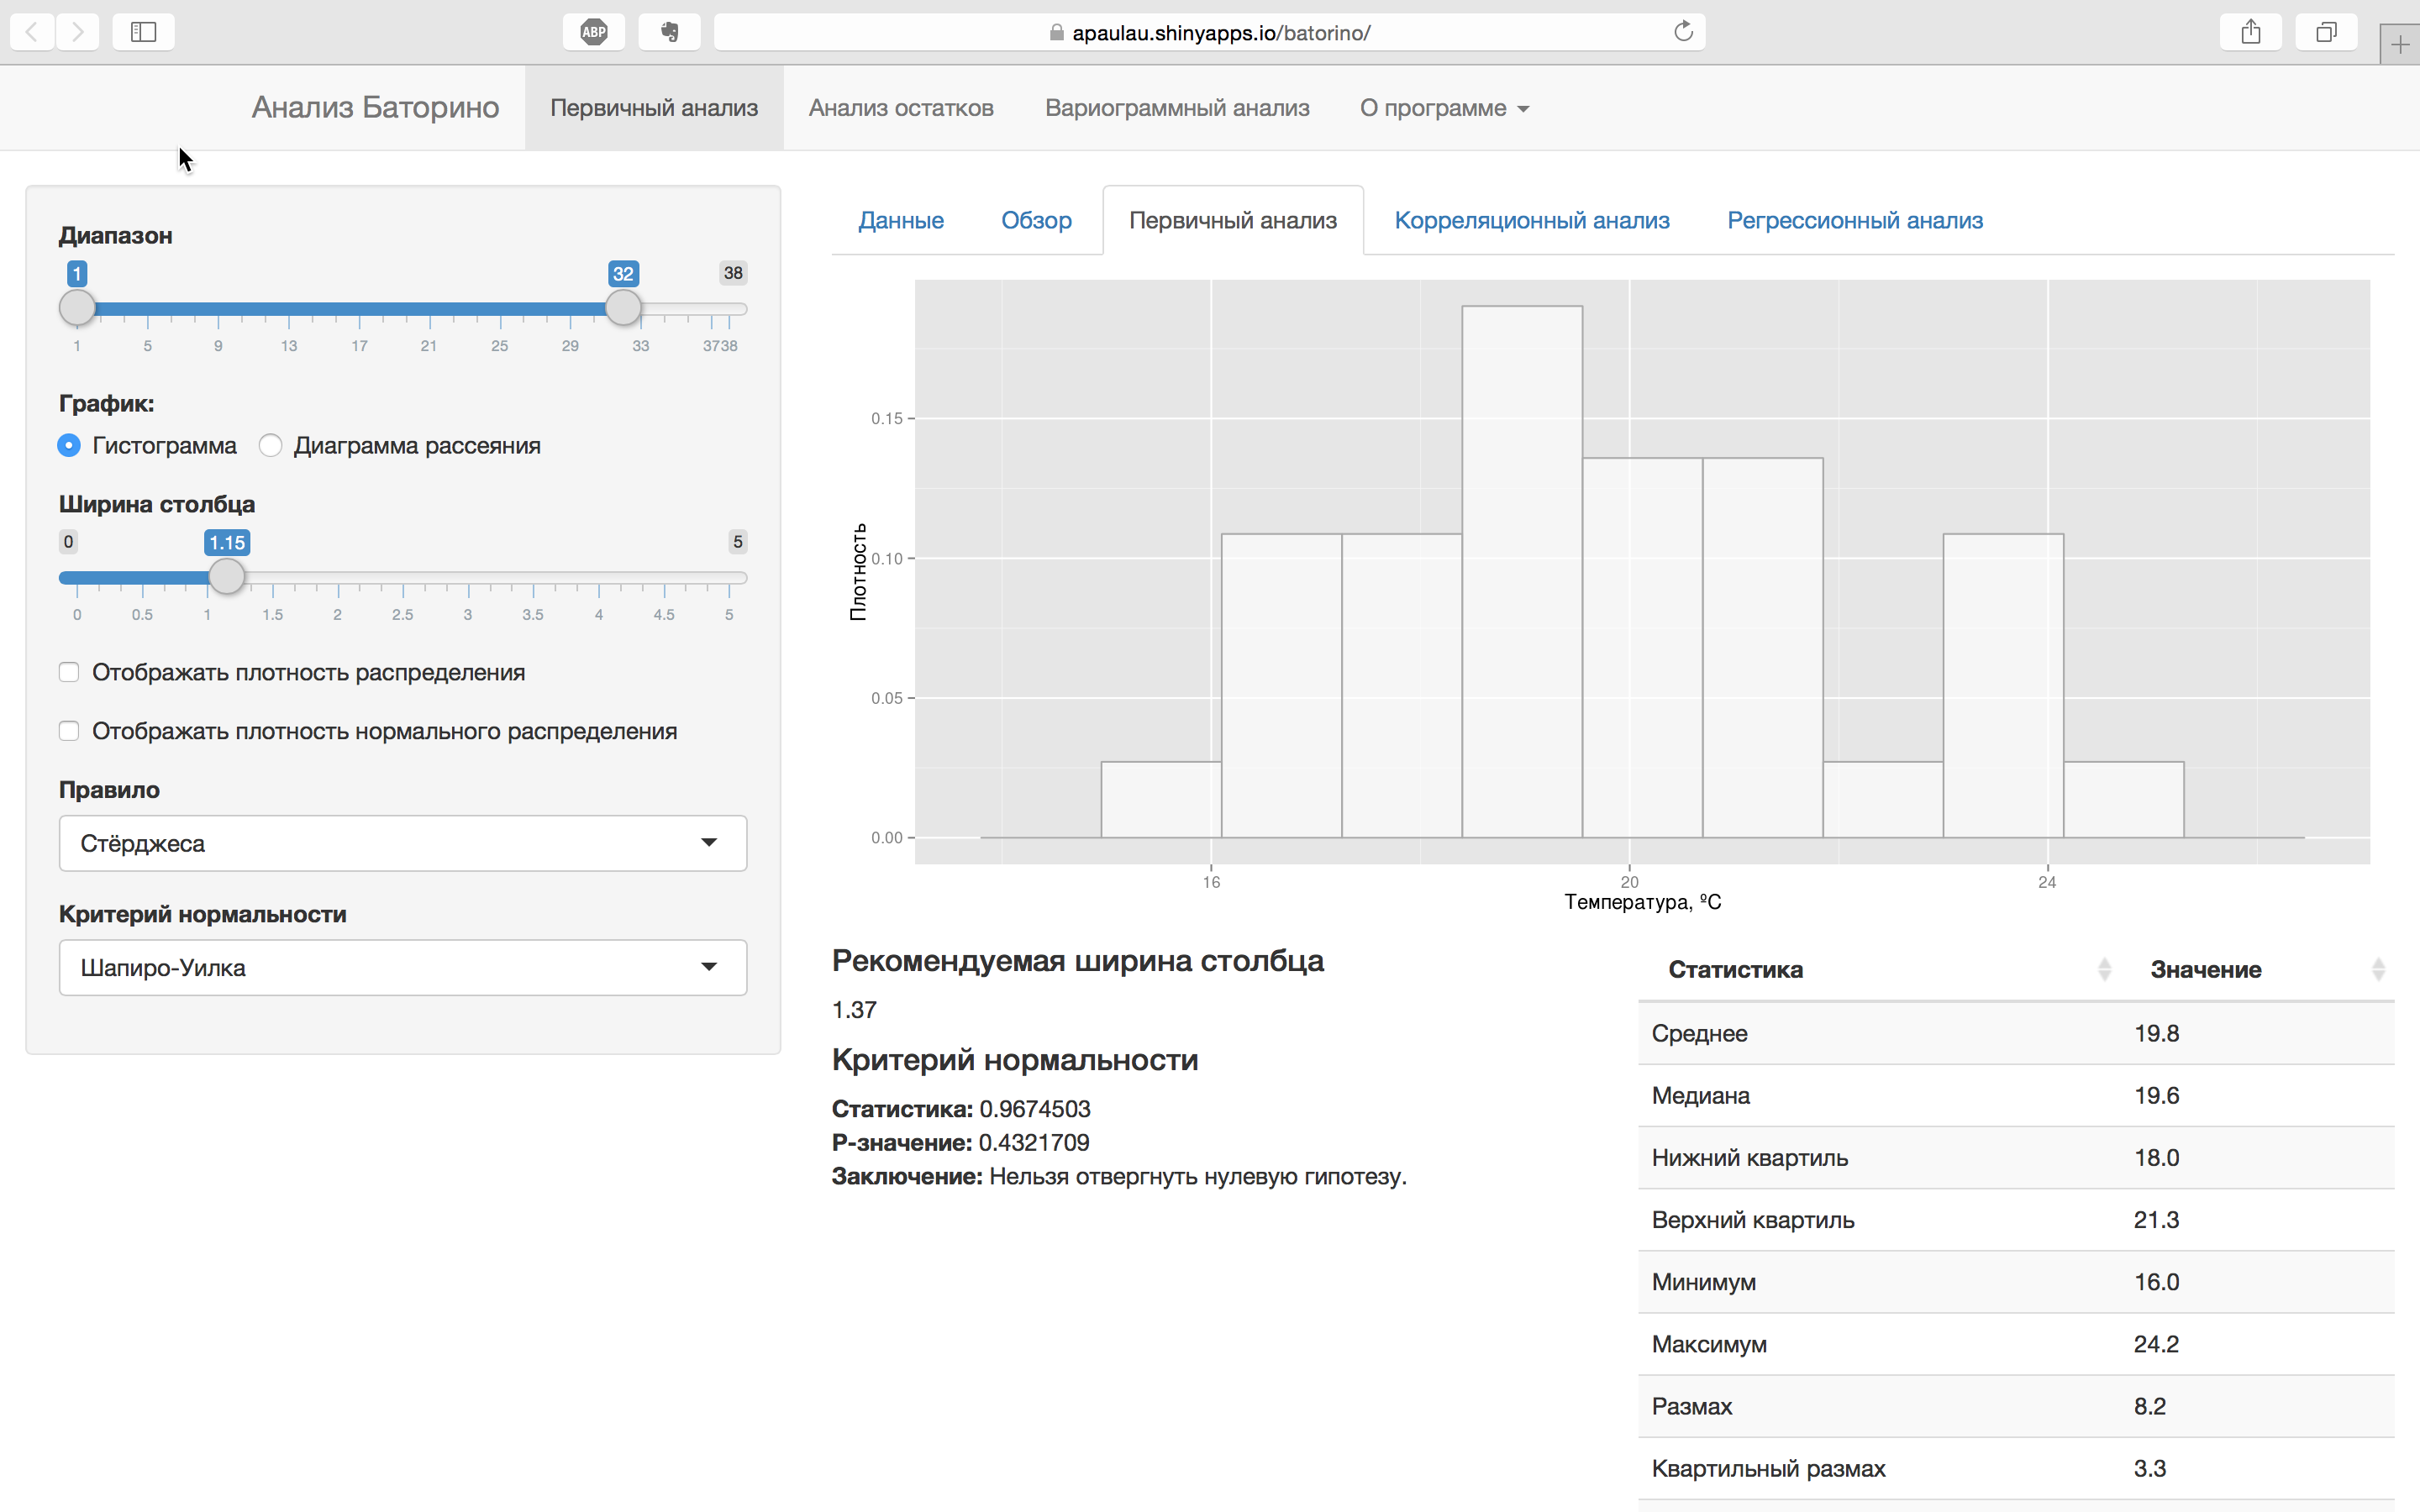
\includegraphics[width=4.5in]{../../figures/static/1_basis.png}
  \end{columns}
\end{frame}

\begin{frame}
  \frametitle{Корреляционный анализ}   % Insert frame title between curly braces
   \begin{columns}[c]
   \column{4.5in}
  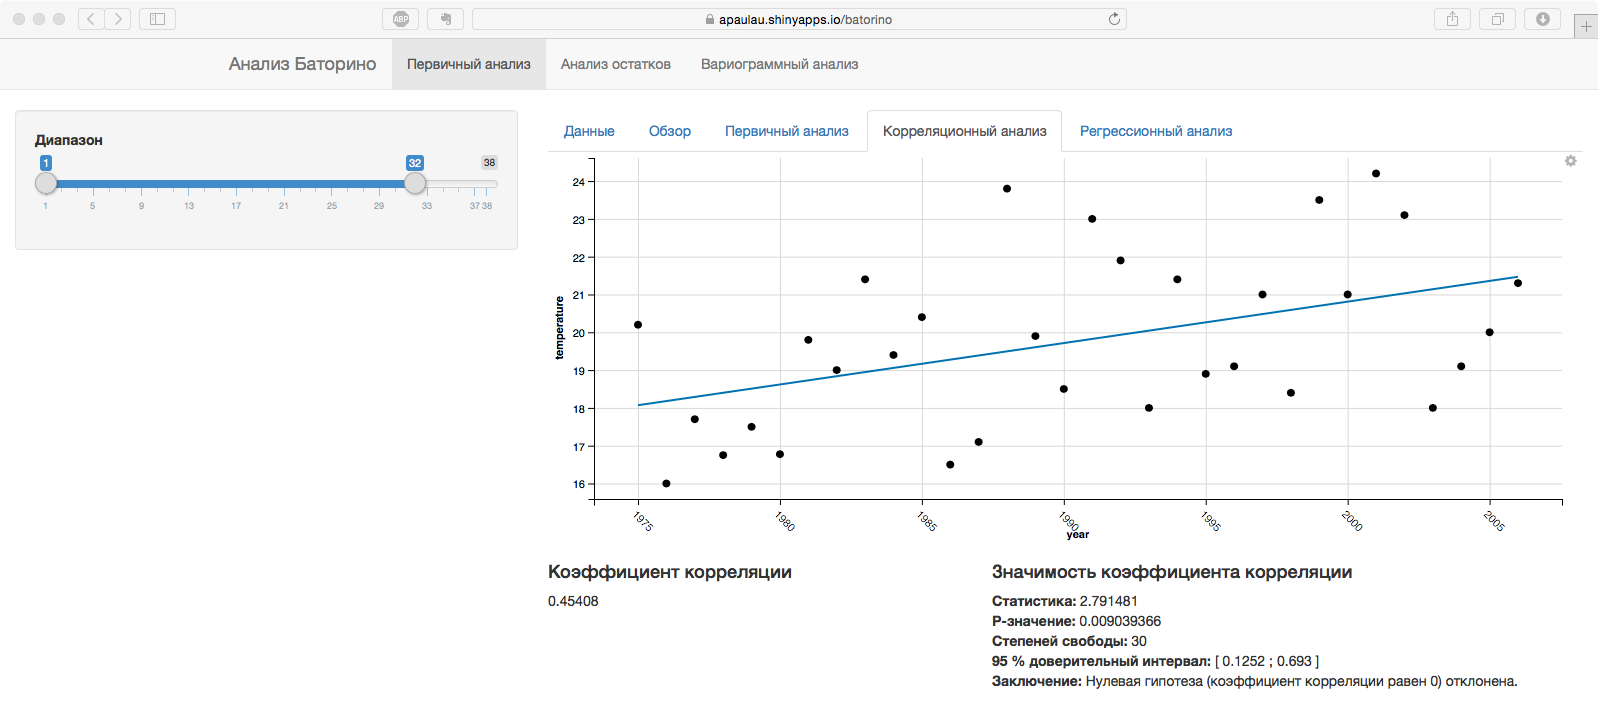
\includegraphics[width=4.5in]{../../figures/static/p_corr.png}
  \end{columns}
\end{frame}

\begin{frame}
  \frametitle{Регрессионный анализ}   % Insert frame title between curly braces
   \begin{columns}[c]
   \column{4.5in}
  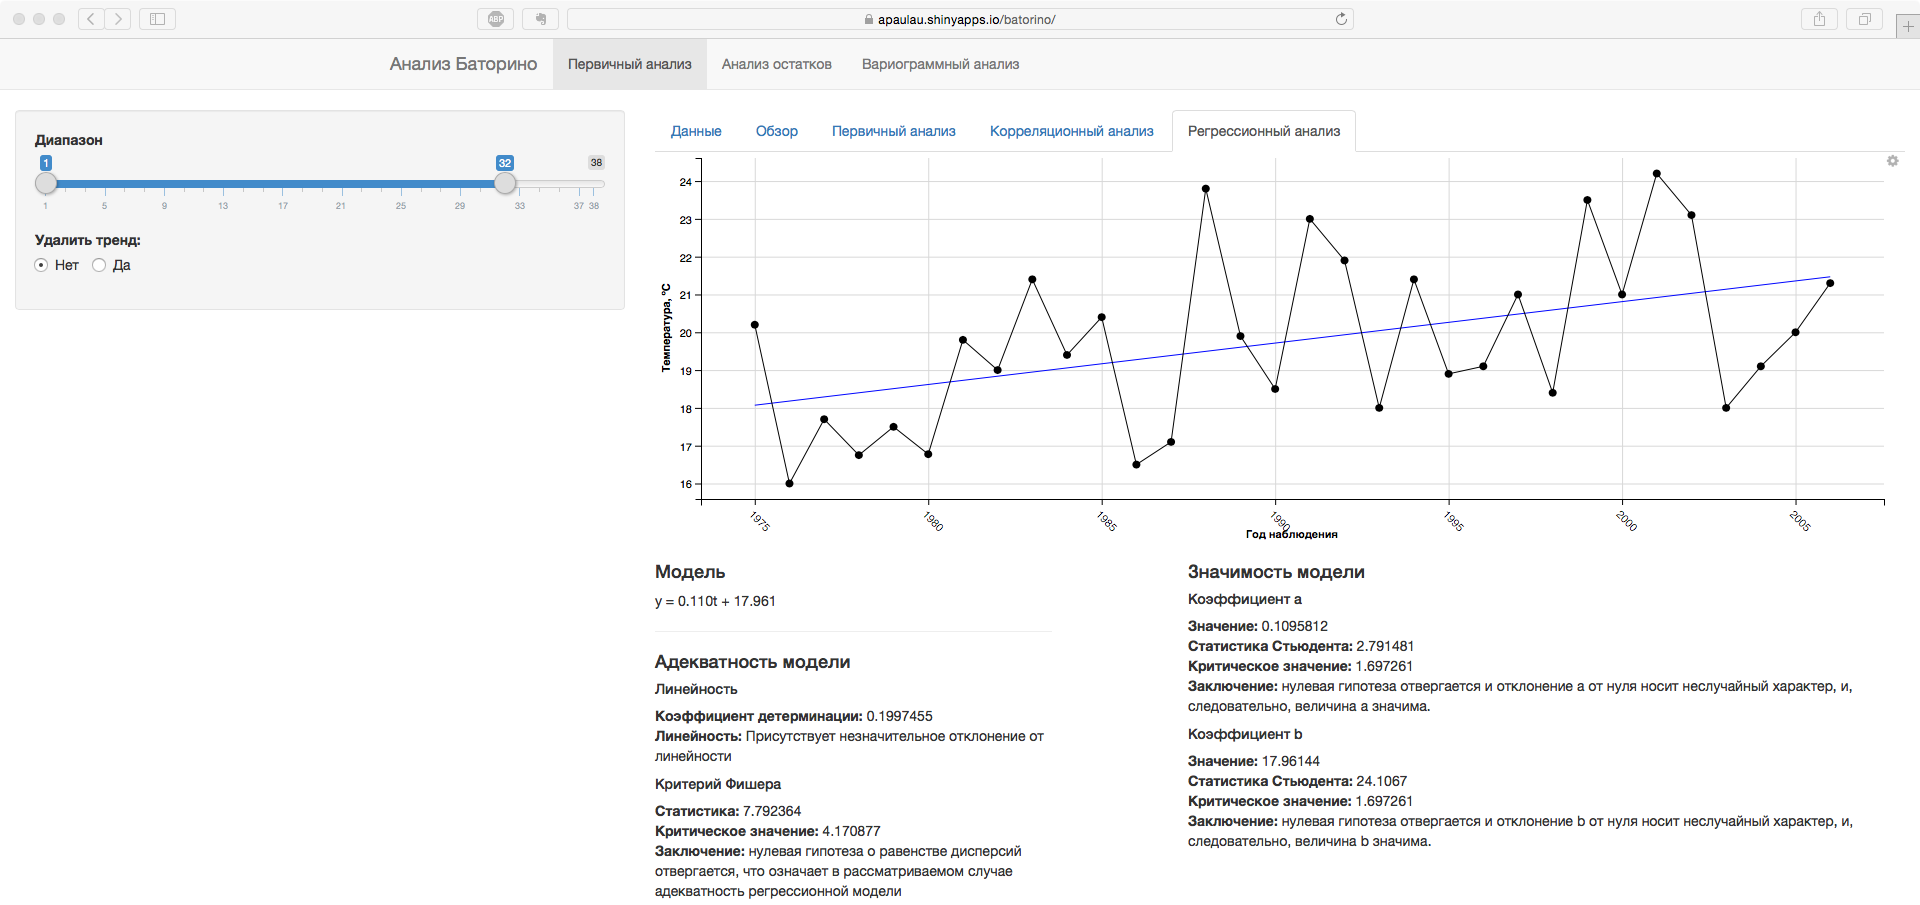
\includegraphics[width=4.5in]{../../figures/static/2_regr.png}
  \end{columns}
\end{frame}

\subsection{Модуль анализа остатков}

\begin{frame}
  \frametitle{Автокорреляционная функция}   % Insert frame title between curly braces
   \begin{columns}[c]
   \column{4.5in}
  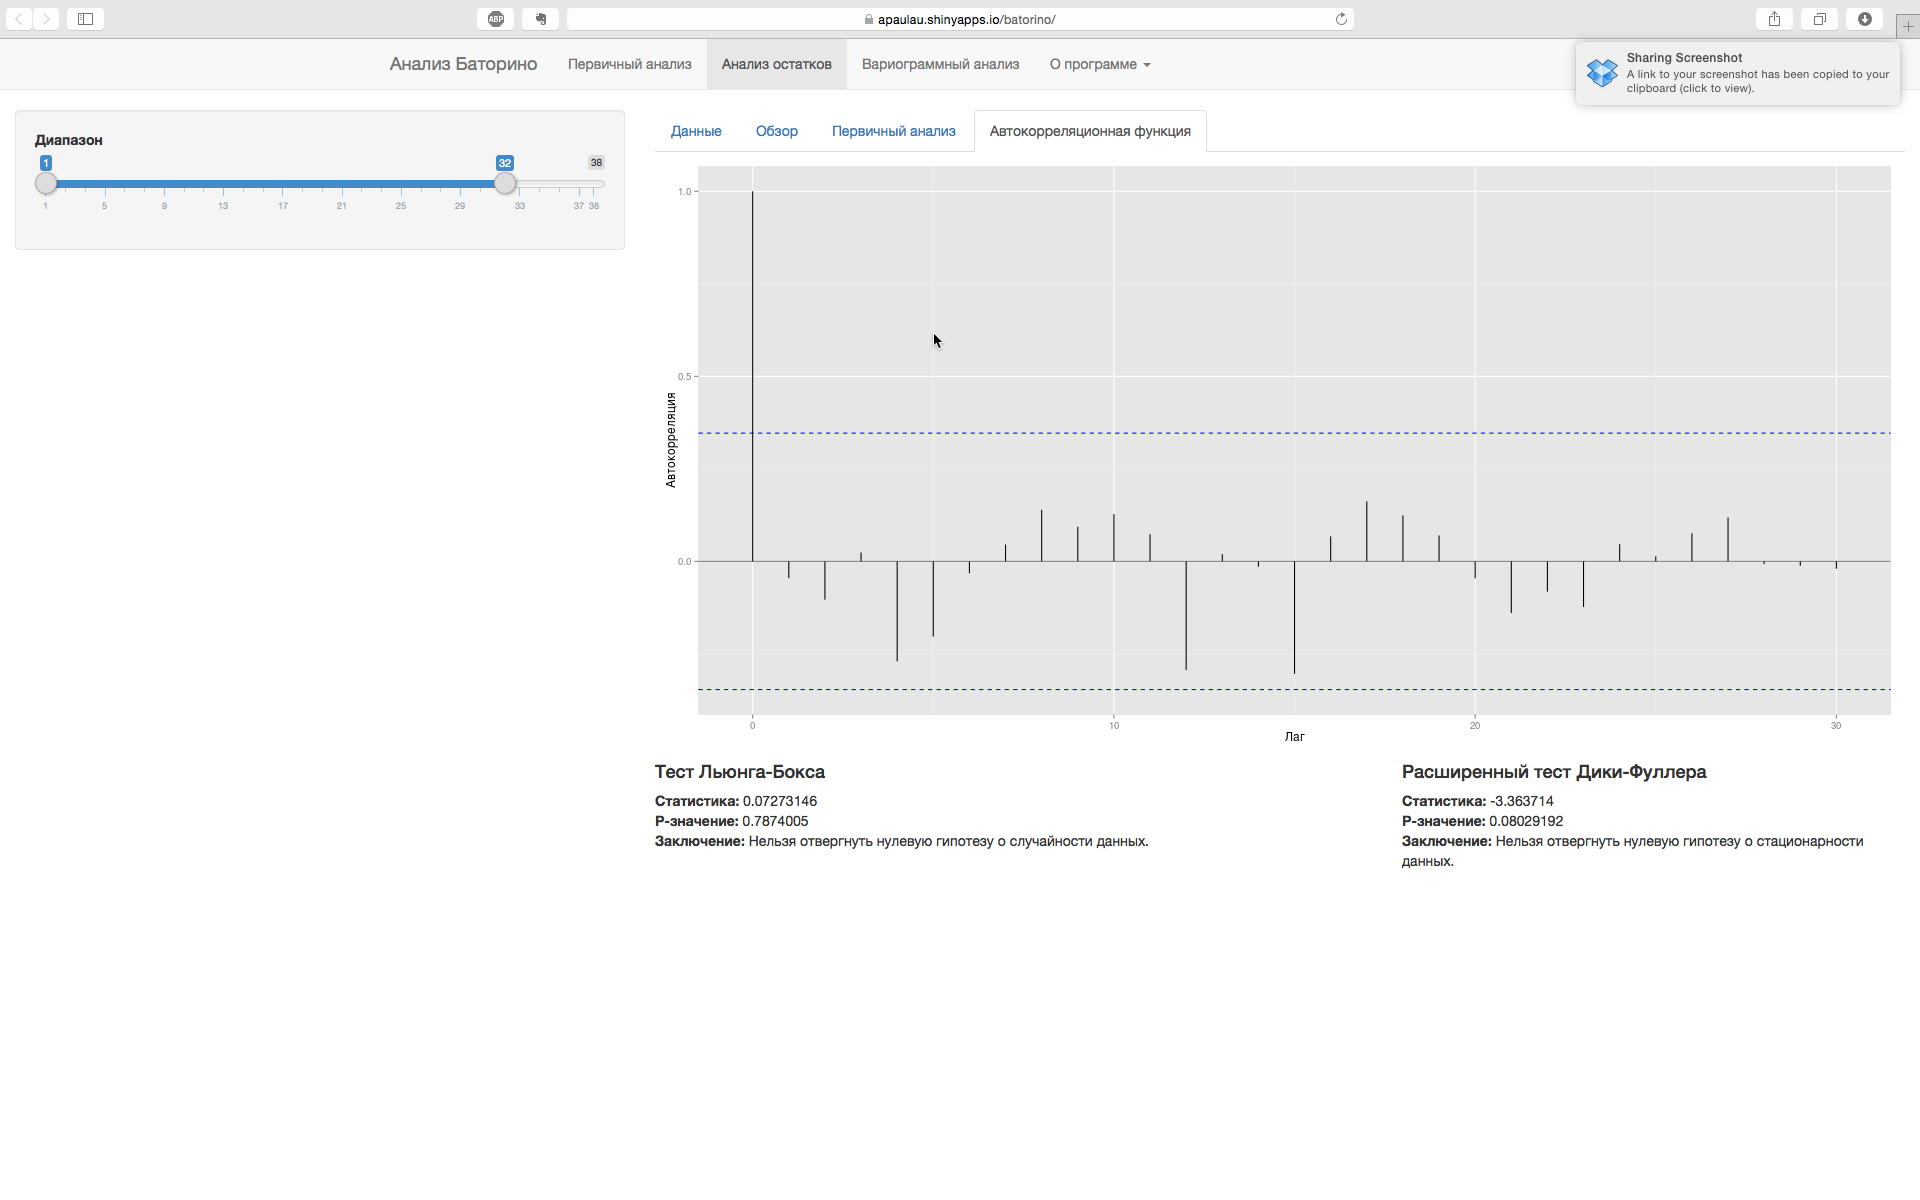
\includegraphics[width=4.5in]{../../figures/static/3_acf.png}
  \end{columns}
\end{frame}

\subsection{Модуль вариограммного анализа}

\begin{frame}
  \frametitle{Возможности по подбору модели вариограммы}   % Insert frame title between curly braces
   \begin{columns}[c]
   \column{4.5in}
  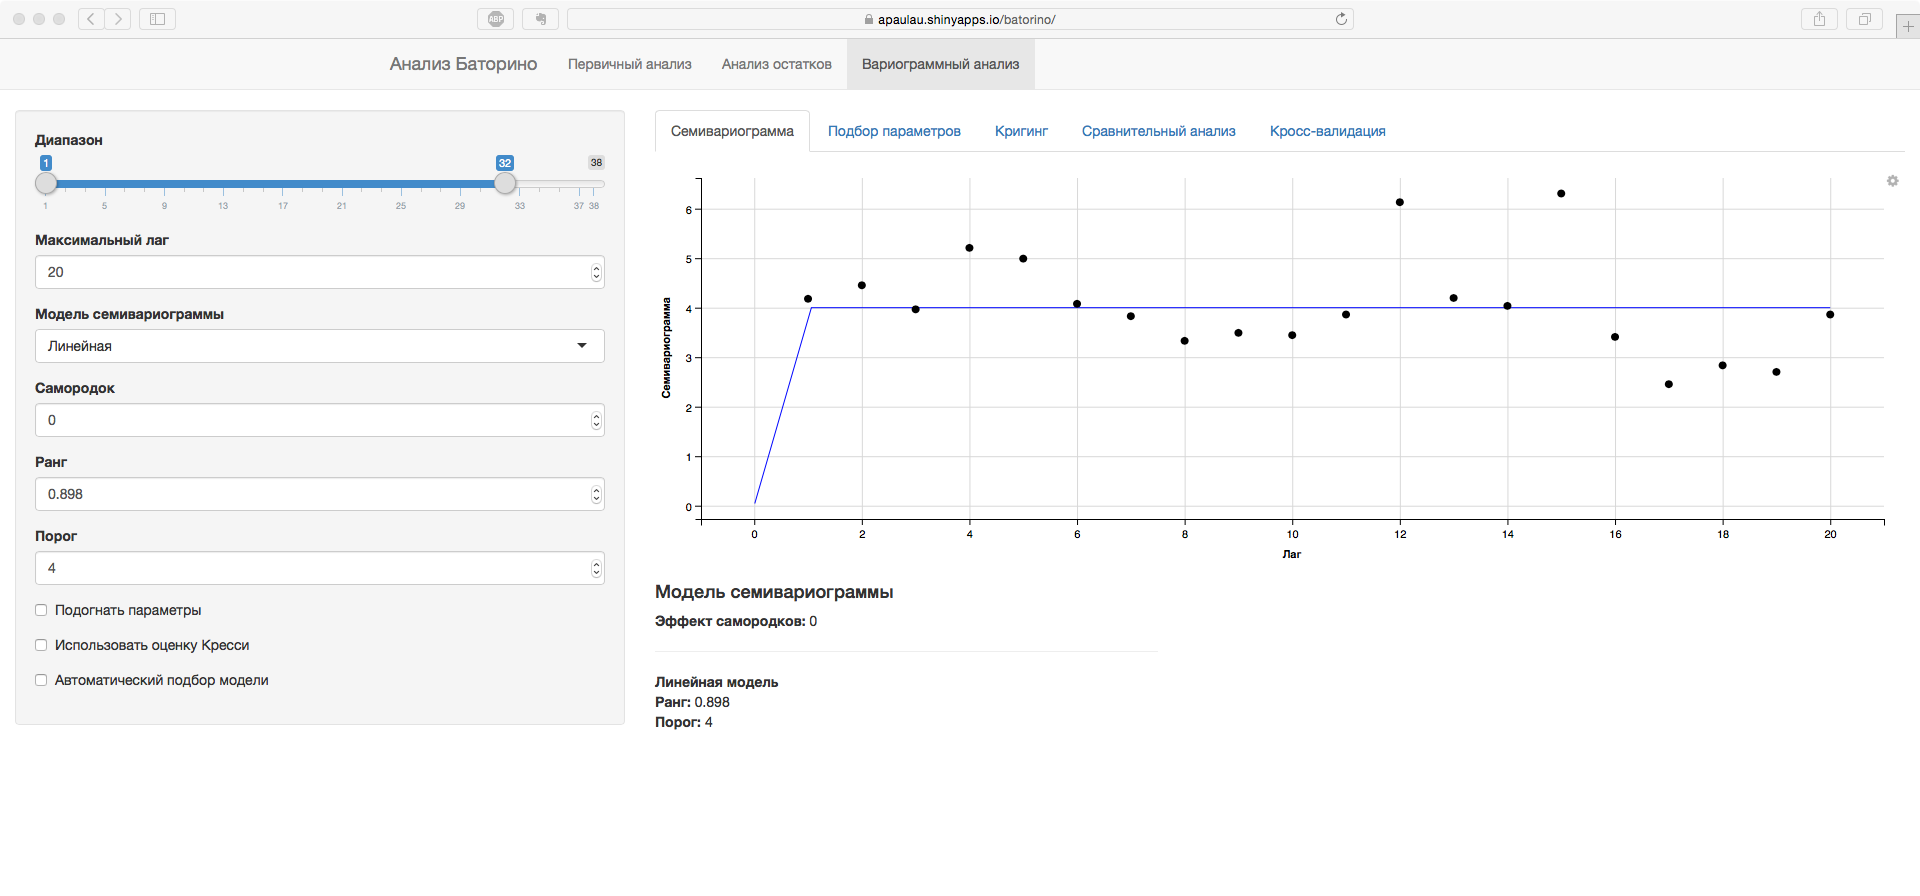
\includegraphics[width=4.5in]{../../figures/static/4_variogram.png}
  \end{columns}
\end{frame}

\begin{frame}
  \frametitle{Подбор параметров модели вариограммы}   % Insert frame title between curly braces
   \begin{columns}[c]
   \column{4.5in}
  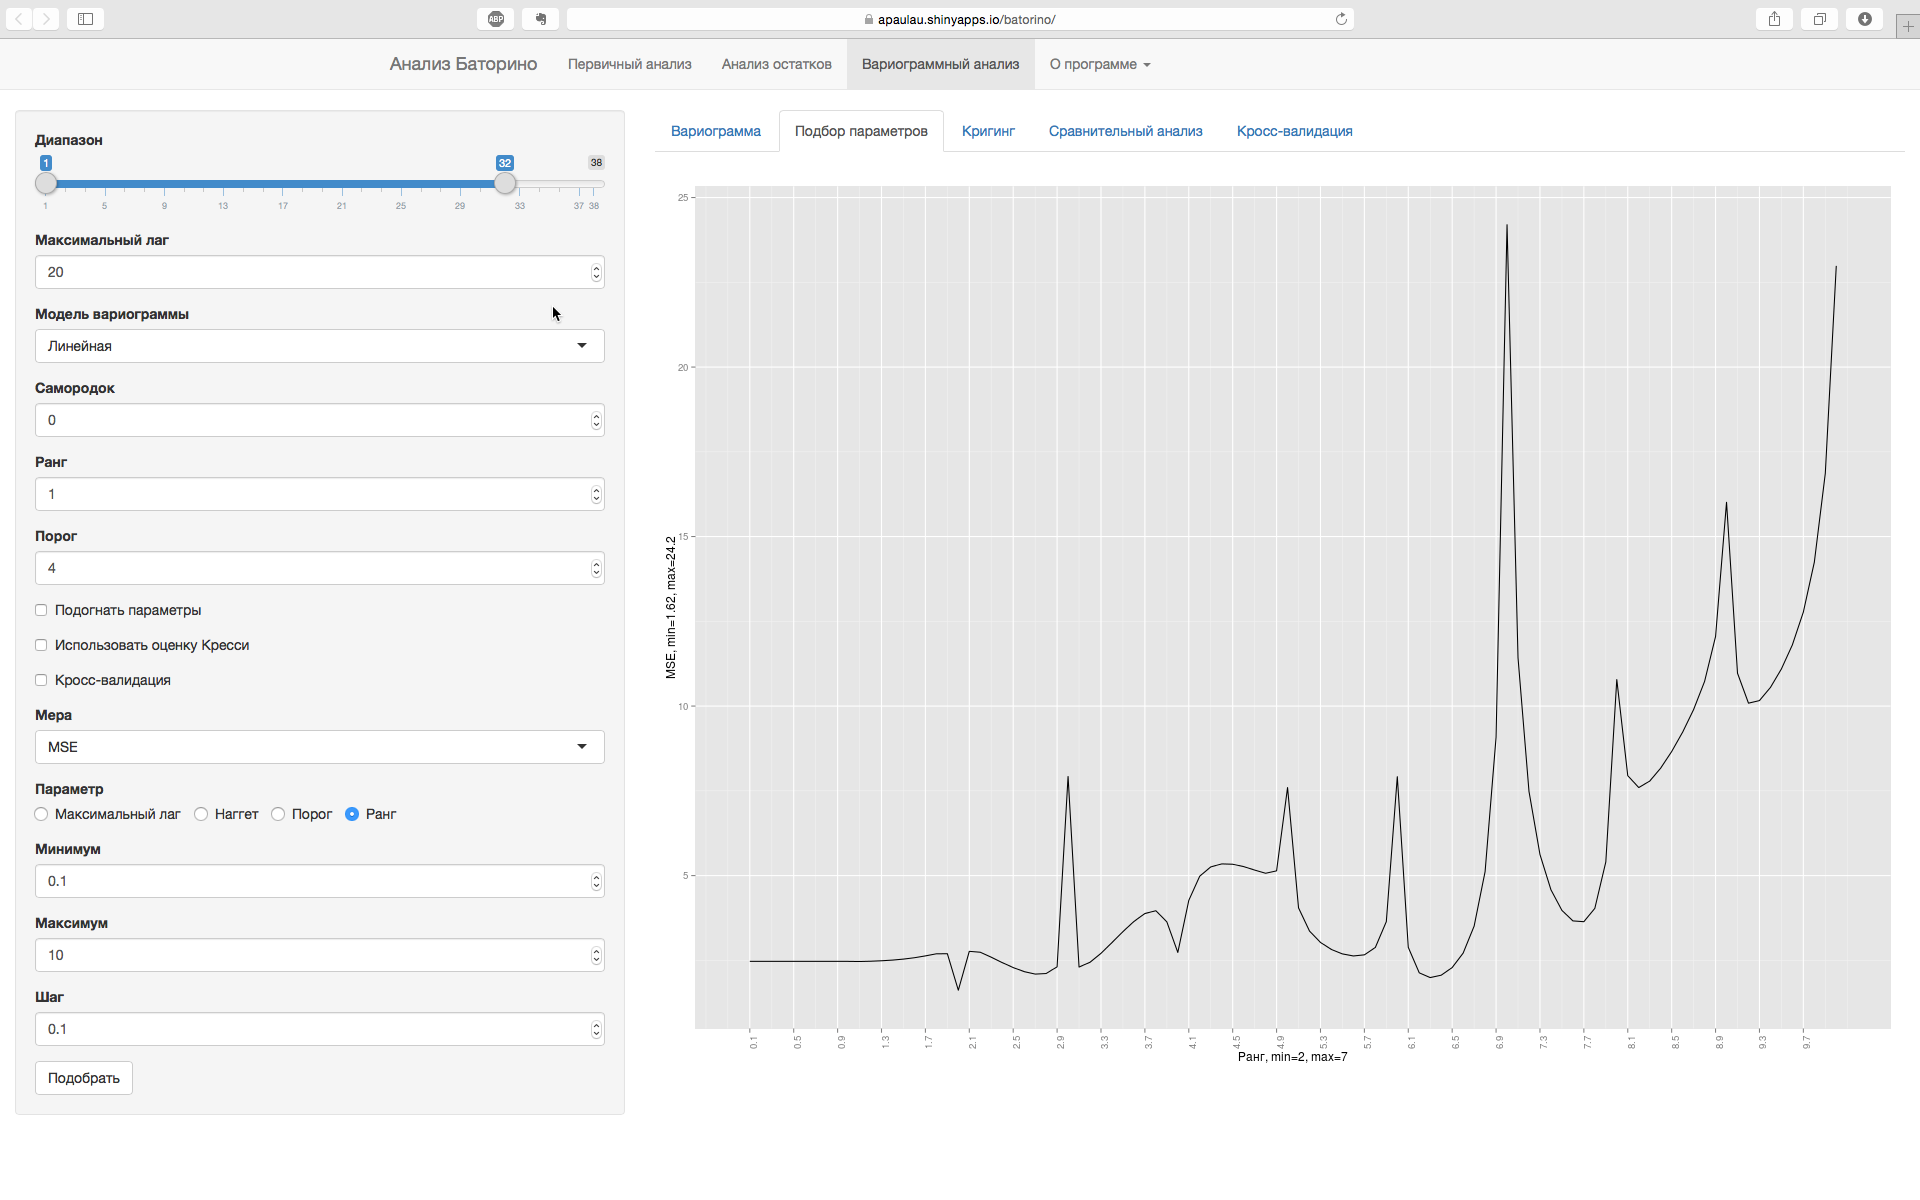
\includegraphics[width=4.5in]{../../figures/static/5_fit.png}
  \end{columns}
\end{frame}

\begin{frame}
  \frametitle{Сравнение прогнозных значений}   % Insert frame title between curly braces
   \begin{columns}[c]
   \column{4.5in}
  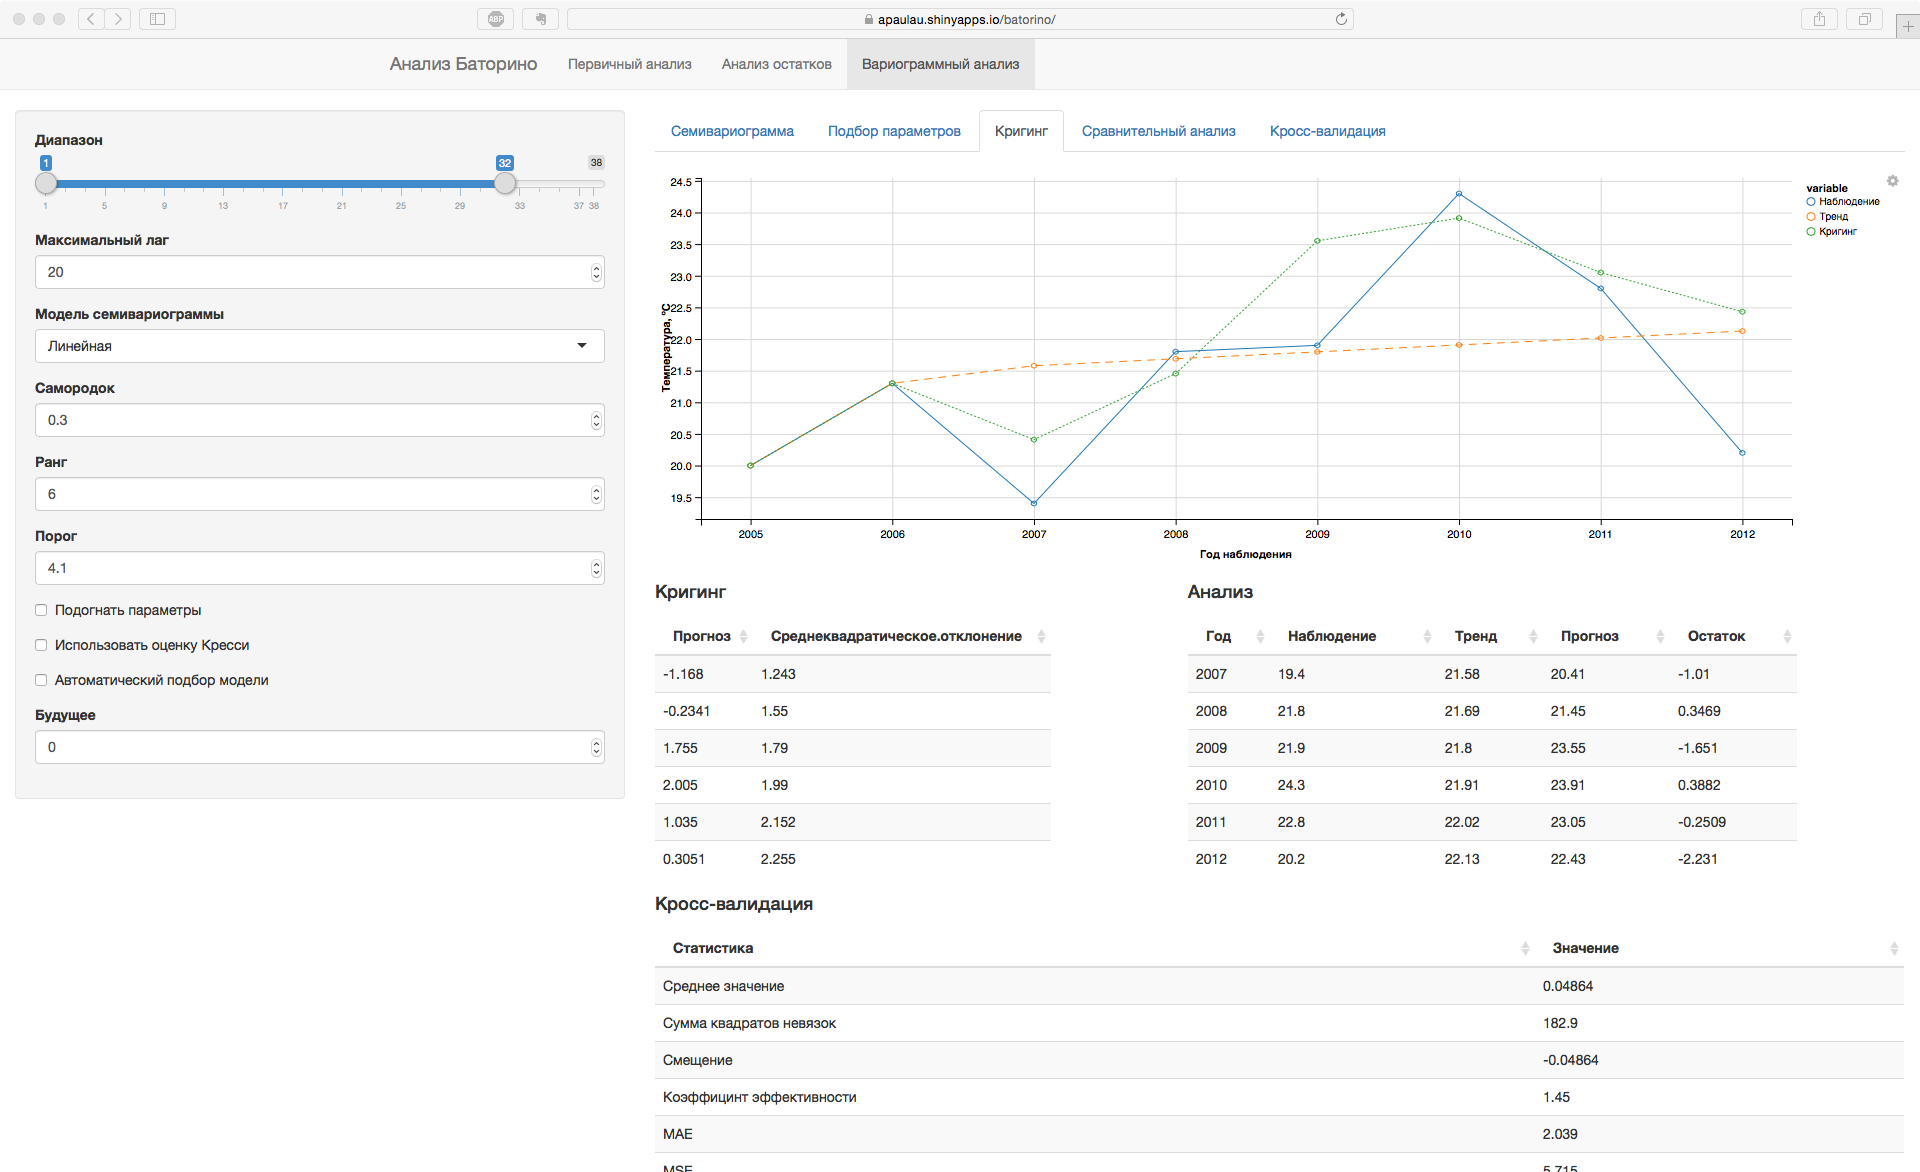
\includegraphics[width=4.5in]{../../figures/static/6_krige.png}
  \end{columns}
\end{frame}

\section{Предварительный анализ}

\begin{frame}
  \frametitle{Исходные данные}   % Insert frame title between curly braces
  \begin{columns}[c]
  \column{2in}  % slides are 3in high by 5in wide
  Исходные данные получены от учебно-научного центра <<Нарочанская биологическая станция им. Г.Г.Винберга>>.

  На рисунке представлена выборка, состоящая из наблюдений за температурой воды в июле месяце в период с 1975 по 2012 годы.
  \column{3in}
  \framebox{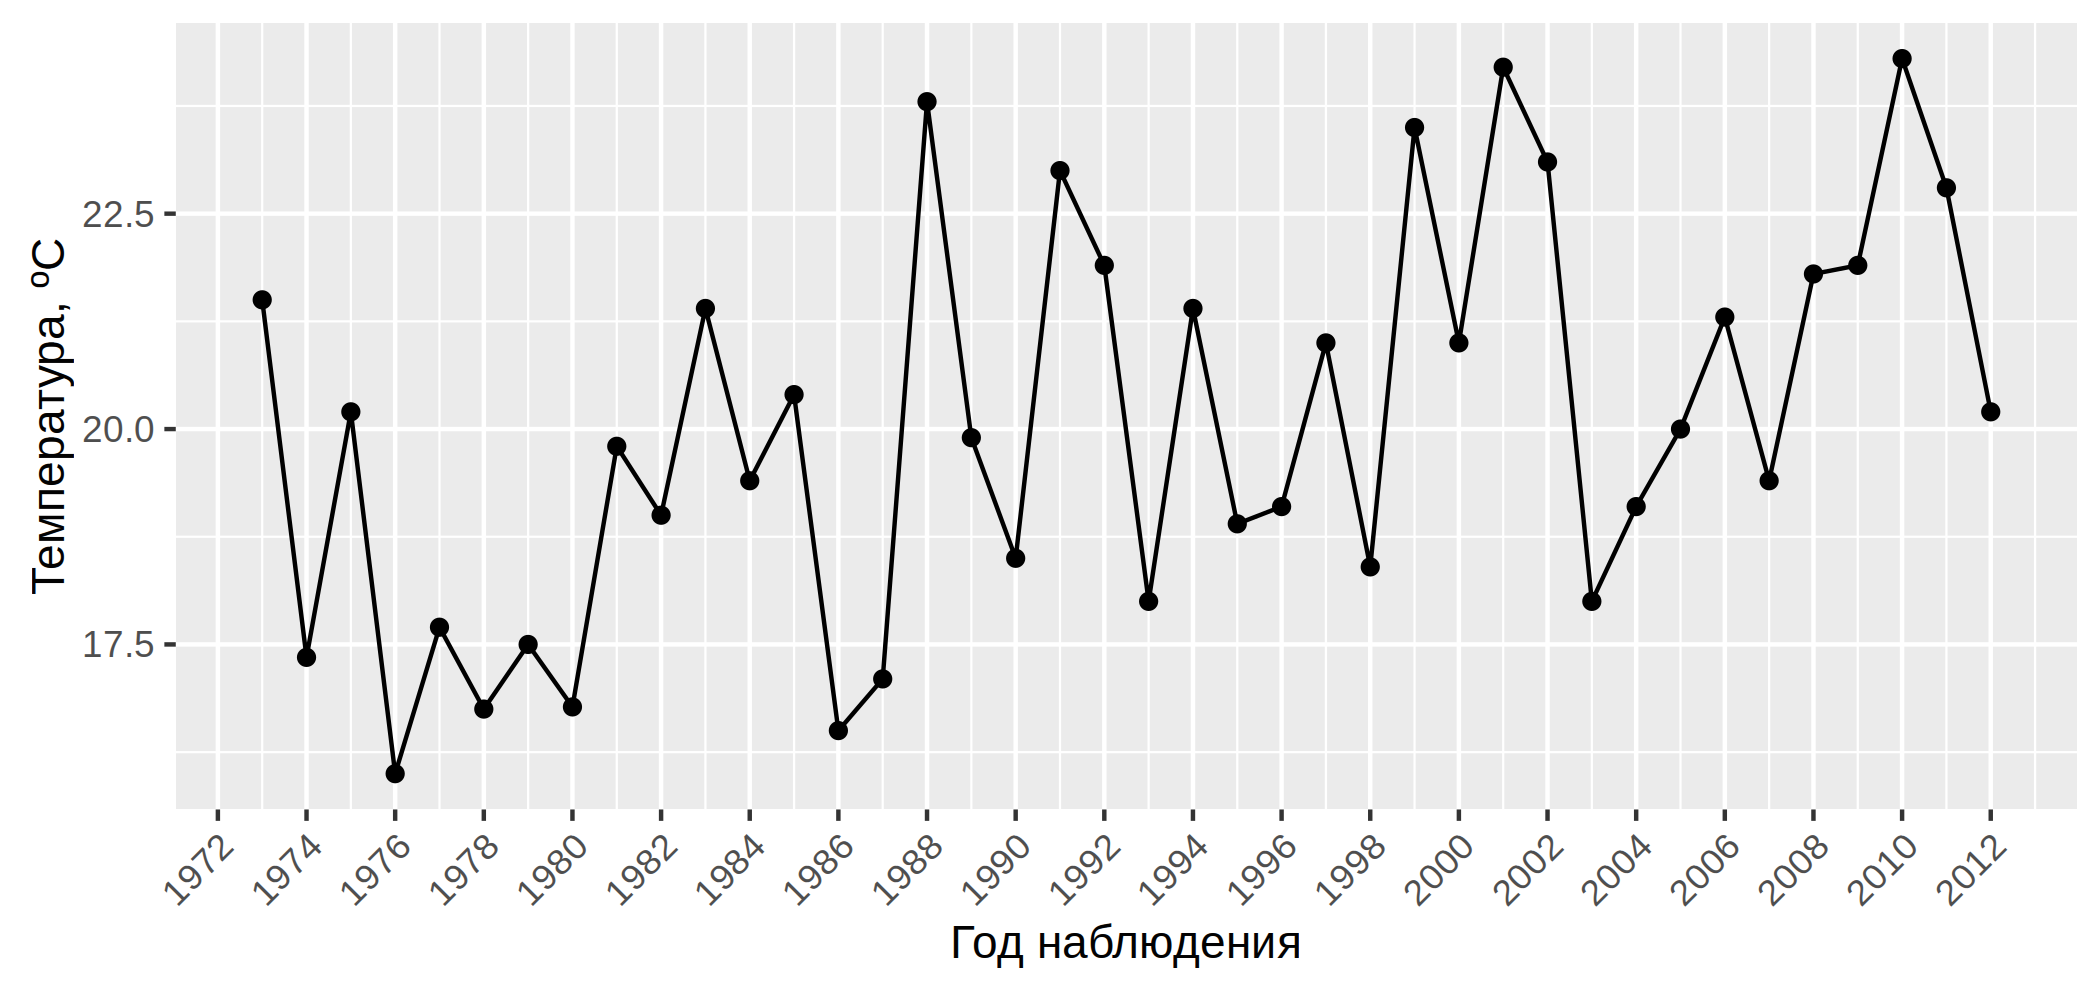
\includegraphics[width=3in]{../../figures/source.png}}
  \end{columns}
\end{frame}

\subsection{Проверка на нормальность}

\begin{frame}
  \frametitle{График квантилей}   % Insert frame title between curly braces
   \begin{columns}[c]
   \column{4.5in}
  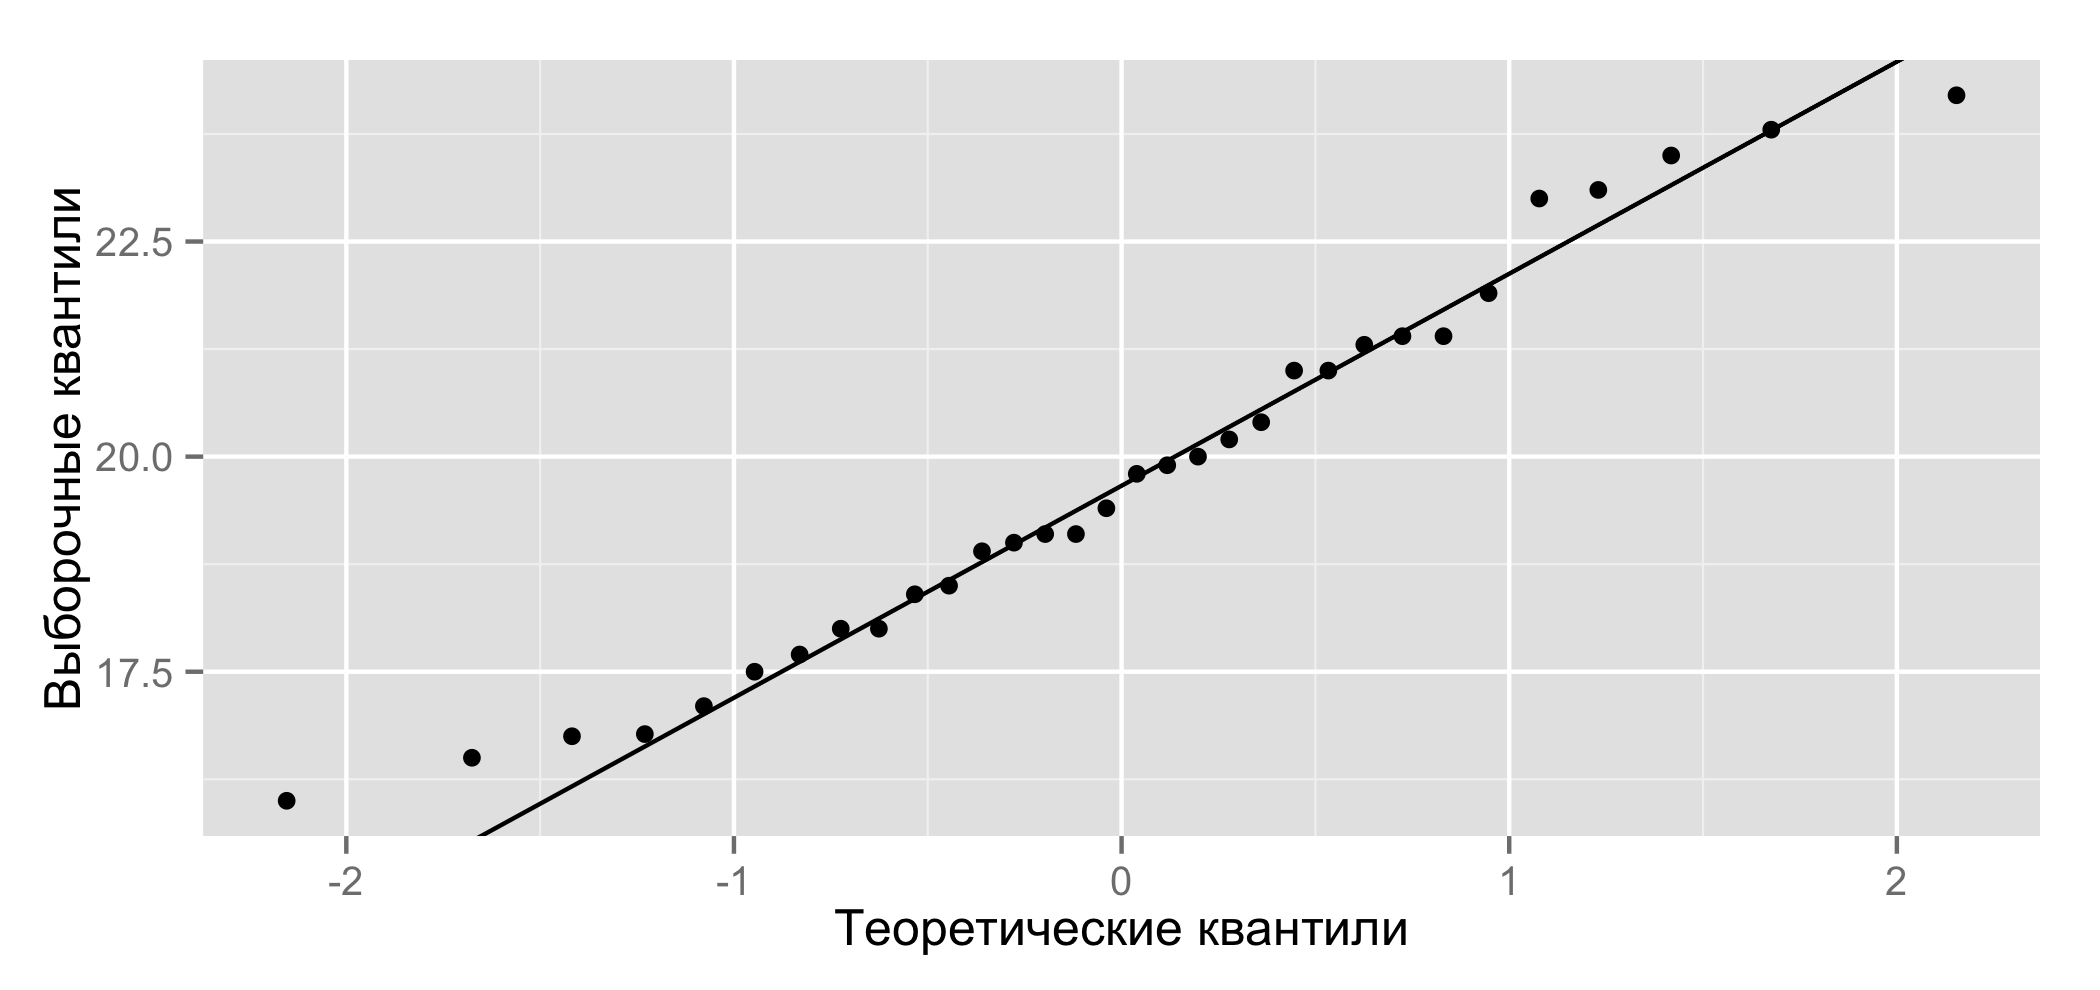
\includegraphics[width=4.5in]{../../figures/original/quantile.png}
  \end{columns}
\end{frame}

\subsection{Корреляционный анализ}

\subsubsection{Проверка наличия зависимости между температурой воды и временем}
\begin{frame}
  \frametitle{Диаграмма рассеяния}   % Insert frame title between curly braces
  \begin{columns}[c]
  \column{2in}  % slides are 3in high by 5in wide
  Выборочный коэффициент корреляции: $ r_{xt} = \characteristic{original}{correlation} $.

  При уровне значимости $ \alpha=0.05 $ коэффициент является значимым
  \column{3in}
  \framebox{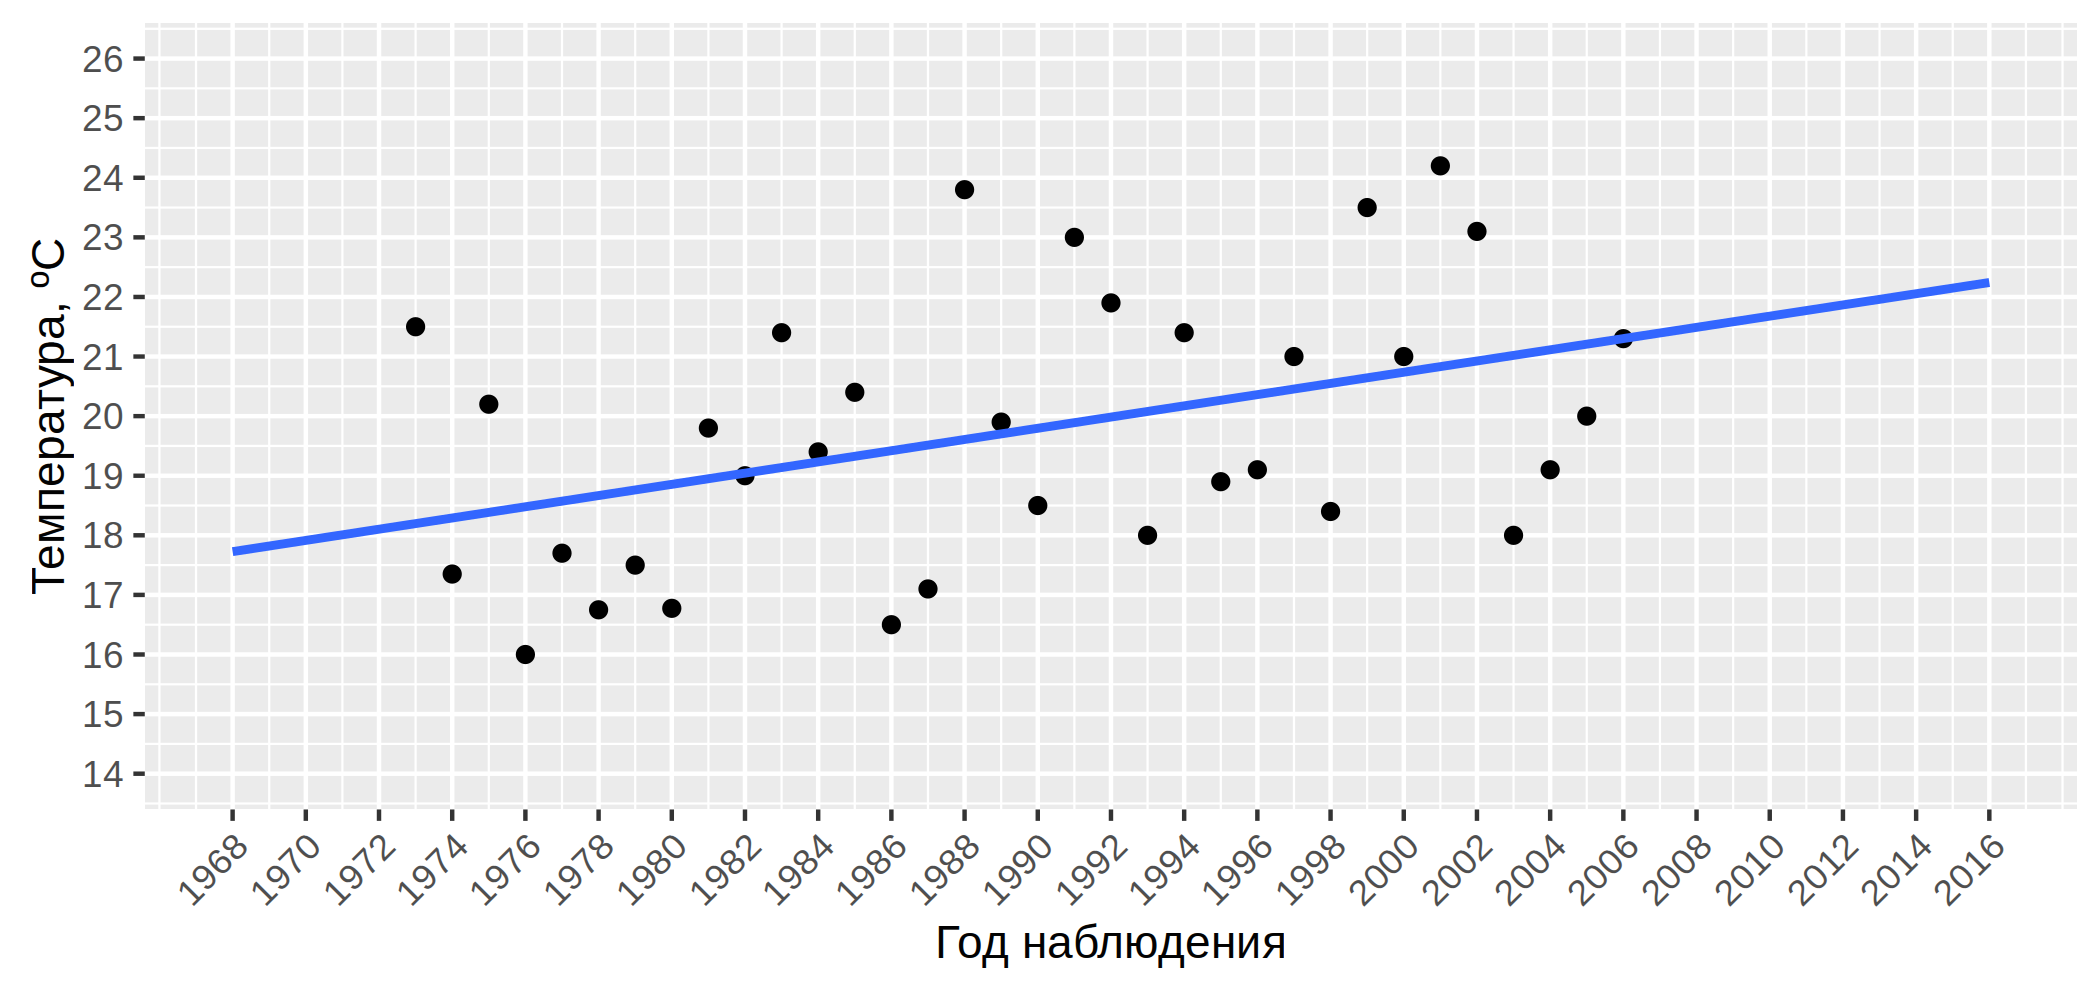
\includegraphics[width=3in]{../../figures/original/scatterplot.png}}
  \end{columns}
\end{frame}

\subsection{Регрессионный анализ}

\subsubsection{Регрессионная модель}
\begin{frame}
  \frametitle{Временной ряд}   % Insert frame title between curly braces
  \begin{columns}[c]
  \column{2in}  % slides are 3in high by 5in wide
  Вид исходного временного ряда: $x(t) = y(t) + \varepsilon(t)$

  Уравнение тренда: $ y(t) = at + b = 0.1014t + 18.0521 $
  \column{3in}
  \framebox{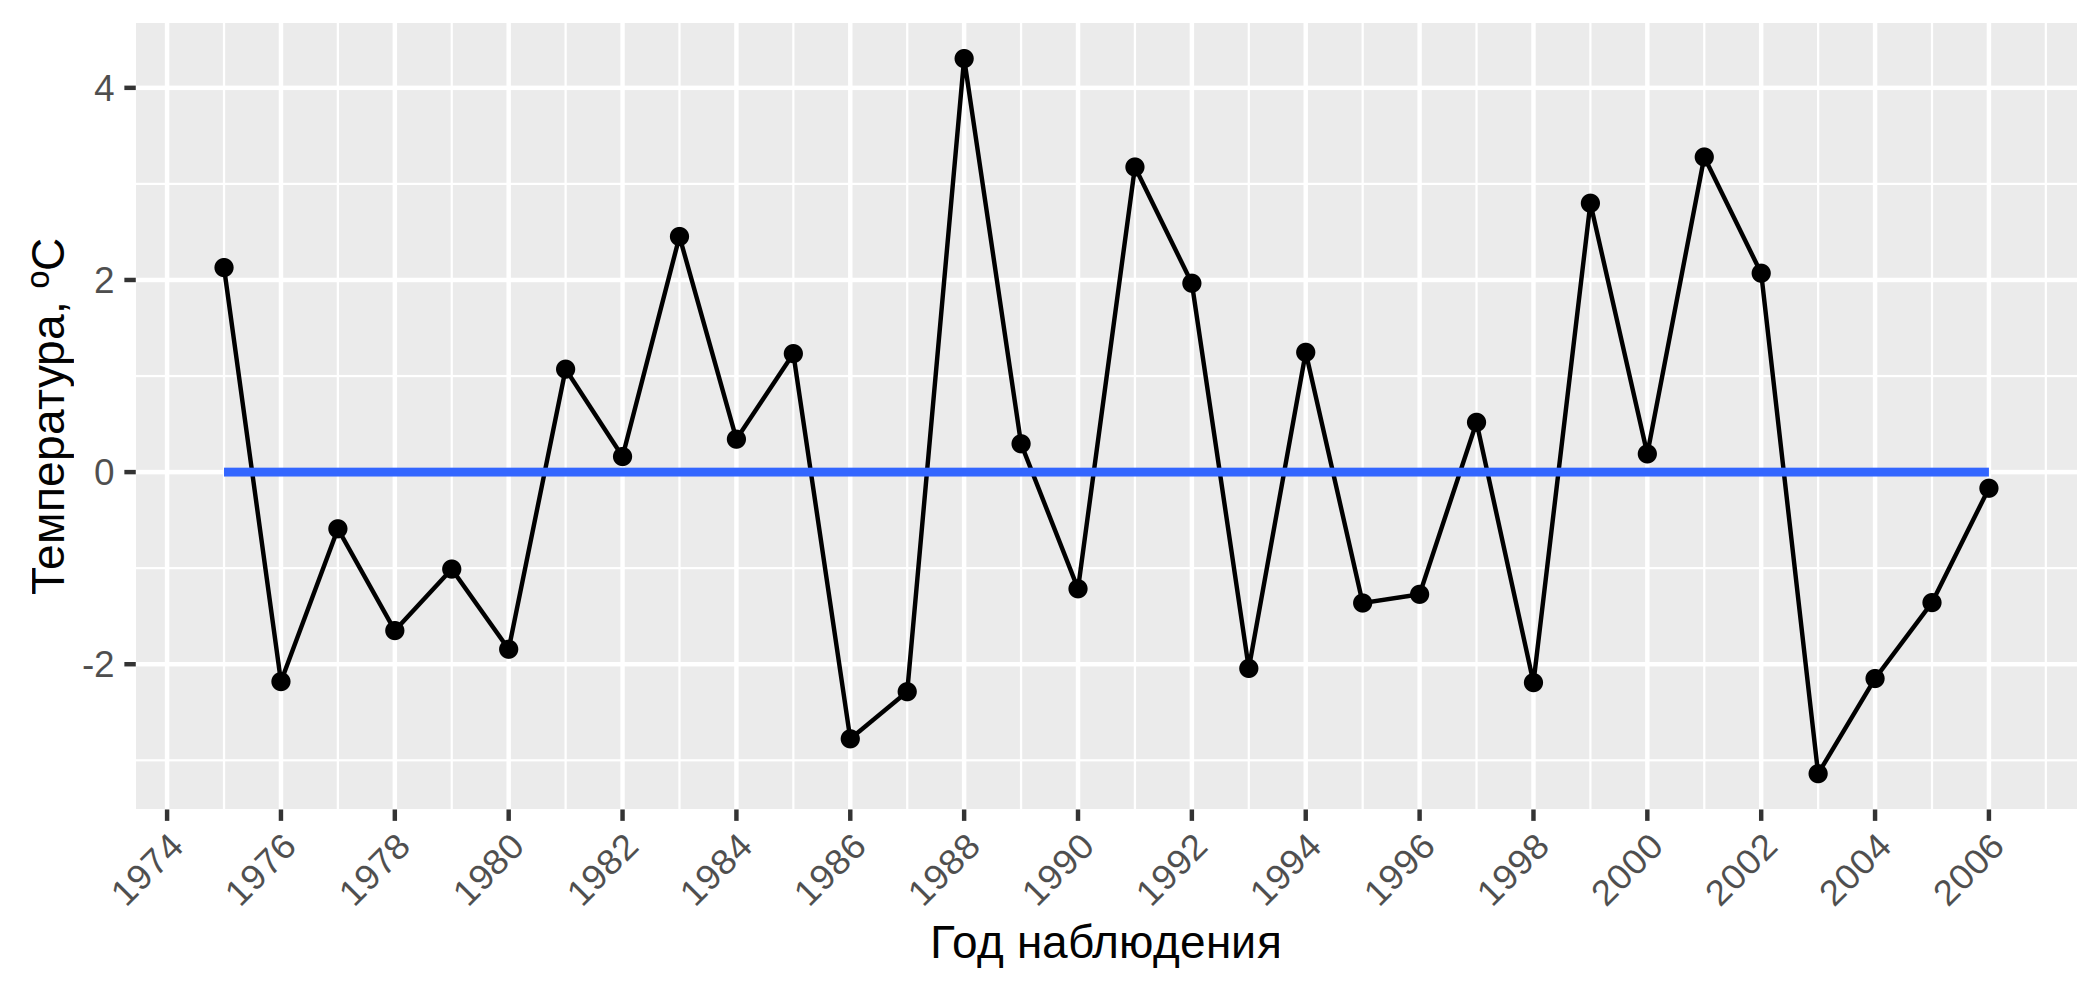
\includegraphics[width=3in]{../../figures/residual/time-series.png}}
  \end{columns}
\end{frame}

\subsubsection{Качество регрессионной модели}
\begin{frame}
  \frametitle{Оценка модели}   % Insert frame title between curly braces
  \begin{itemize}
    \item С помощью критерия Стьюдента доказана значимость коэффициентов регрессионной модели
    \item F-критерий Фишера при уровне значимости $ \alpha = 0.05 $ показал адекватность модели
    \item Точность модели невысока, поскольку коэффициент детерминации $ \eta^2_{x(t)} = 0.275 $
  \end{itemize}
\end{frame}

% \subsection{Анализ остатков}

% \begin{frame}
%   \frametitle{Автокорреляционная функция}   % Insert frame title between curly braces
%    \begin{columns}[c]
%    \column{4.5in}
%   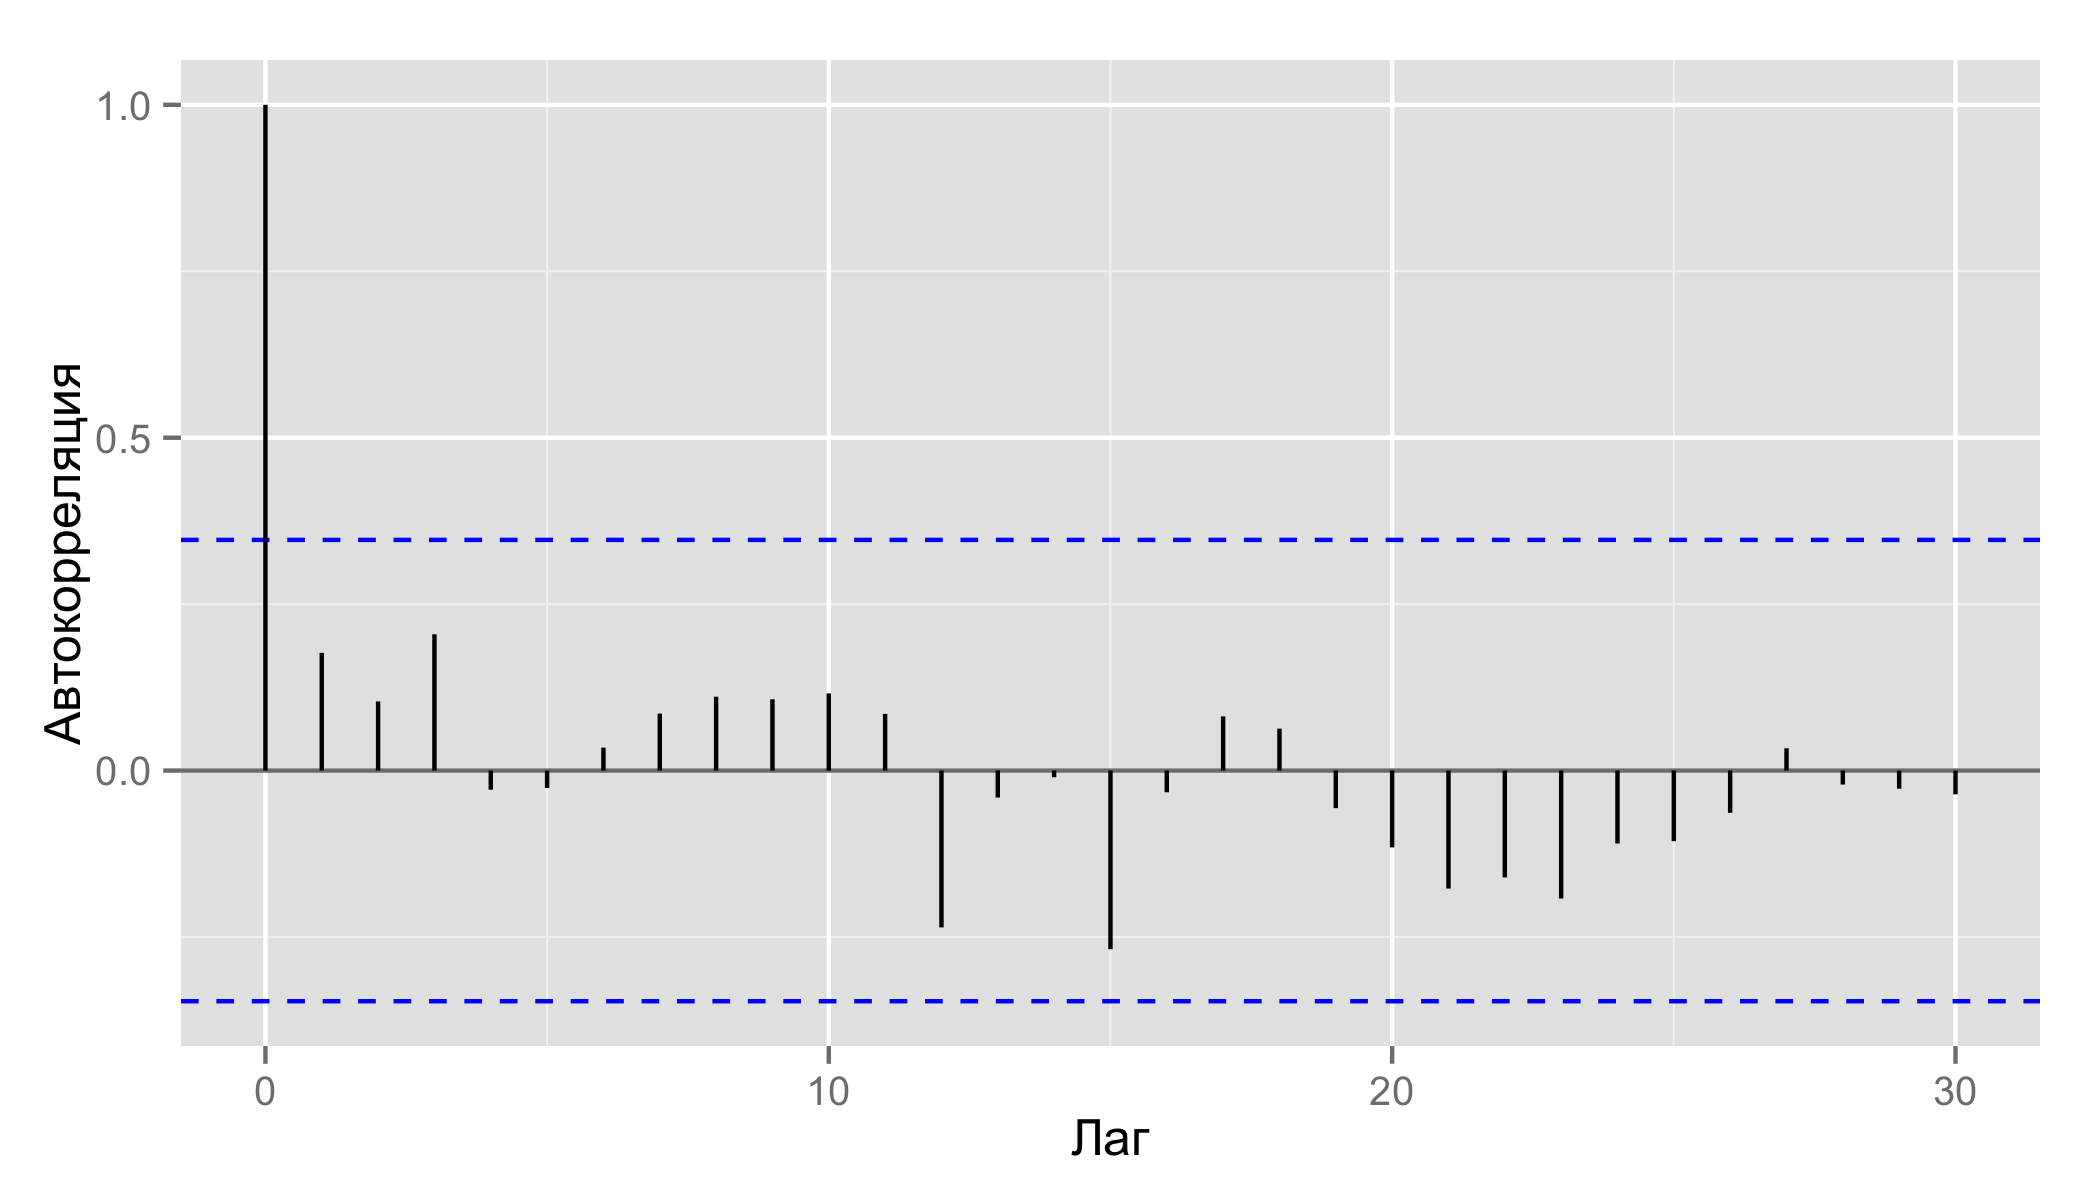
\includegraphics[width=4.5in]{../../figures/residual/acf.png}
%   \end{columns}
% \end{frame}

\section{Вариограммный анализ}

\subsection{Теория}

\begin{frame}
  \frametitle{Оценка вариограммы}   % Insert frame title between curly braces
  В качестве оценки вариограммы рассмотривается статистика, предложенная Матероном:
  \begin{equation}
    2 \tilde{\gamma}(h) = \frac{1}{n - h} \sum_{t = 1}^{n - h}(X(t + h) - X(t))^2, \quad h = \overline{0, n - 1},
  \end{equation}
\end{frame}

\begin{frame}
  \frametitle{Первые два момента оценки вариограммы}   % Insert frame title between curly braces
\begin{Theorem}
  Для оценки $ 2 \tilde{\gamma}(h) $ имеют место следующие соотношения:
  \begin{equation*}
    E \{2 \tilde{\gamma}(h) \} = 2 \gamma(h), % DIRTY HACK
  \end{equation*}
  \begin{equation*}
    cov(2 \tilde{\gamma}(h_1), 2 \tilde{\gamma}(h_2)) =
  \end{equation*}
  \begin{equation*}
    = \frac{2}{(n - h_1)(n - h_2)} \sum_{t = 1}^{n - h_1}\sum_{s = 1}^{n - h_2} (\gamma(t - h_2 - s) + \gamma(t + h_1 - s) - \gamma(t - s) - \gamma(t + h_1 - s - h_2))^2,
  \end{equation*}
  \begin{equation*}
    V \{ 2 \tilde{\gamma}(h) \} = \frac{2}{(n-h)^2}\sum_{t,s = 1}^{n - h} ( \gamma(t - h - s) + \gamma(t + h - s) - 2\gamma(t - s) )^2,
  \end{equation*}
  где $ \gamma(h), h \in \mathbb{Z} $, --- семивариограмма процесса $ X(t), t \in \mathbb{Z}$, $ h, h_1, h_2 = \overline{0, n - 1} $.
\end{Theorem}
\end{frame}

\begin{frame}
  \frametitle{Асимптотическое поведение оценки вариограммы}   % Insert frame title between curly braces
  \begin{Theorem}
  Если имеет место соотношение
  \begin{equation*}
    \sum_{h = -\infty}^{+\infty} \vert \gamma(h) \vert < +\infty, \text{то}
  \end{equation*}
  \begin{equation*}
    \lim_{n \to \infty} (n - \min\{ h_1, h_2 \}) cov\{ 2 \tilde{\gamma}(h_1), 2 \tilde{\gamma}(h_2) \} = % DIRTY HACK
  \end{equation*}
  \begin{equation*}
    = 2 \sum_{m = -\infty}^{+\infty} \gamma(m - h_2) + \gamma(m + h_1) - \gamma(m) - \gamma(m + h_1 - h_2))^2,
  \end{equation*}
  \begin{equation*}
    \lim_{n \to \infty} (n - h) V\{ 2 \tilde{\gamma}(h) \} = 2 \sum_{m = -\infty}^{+\infty} \gamma(m - h) + \gamma(m + h) - 2 \gamma(m))^2.
  \end{equation*}
  где $ \gamma(h), h \in \mathbb{Z} $, --- семивариограмма процесса $ X(t), t \in \mathbb{Z}$, $ h, h_1, h_2 = \overline{0, n - 1} $.
\end{Theorem}
\end{frame}

\subsection{Вариограмма}

\begin{frame}
  \frametitle{График экспериментальной вариограммы}   % Insert frame title between curly braces
   \begin{columns}[c]
   \column{4.5in}
  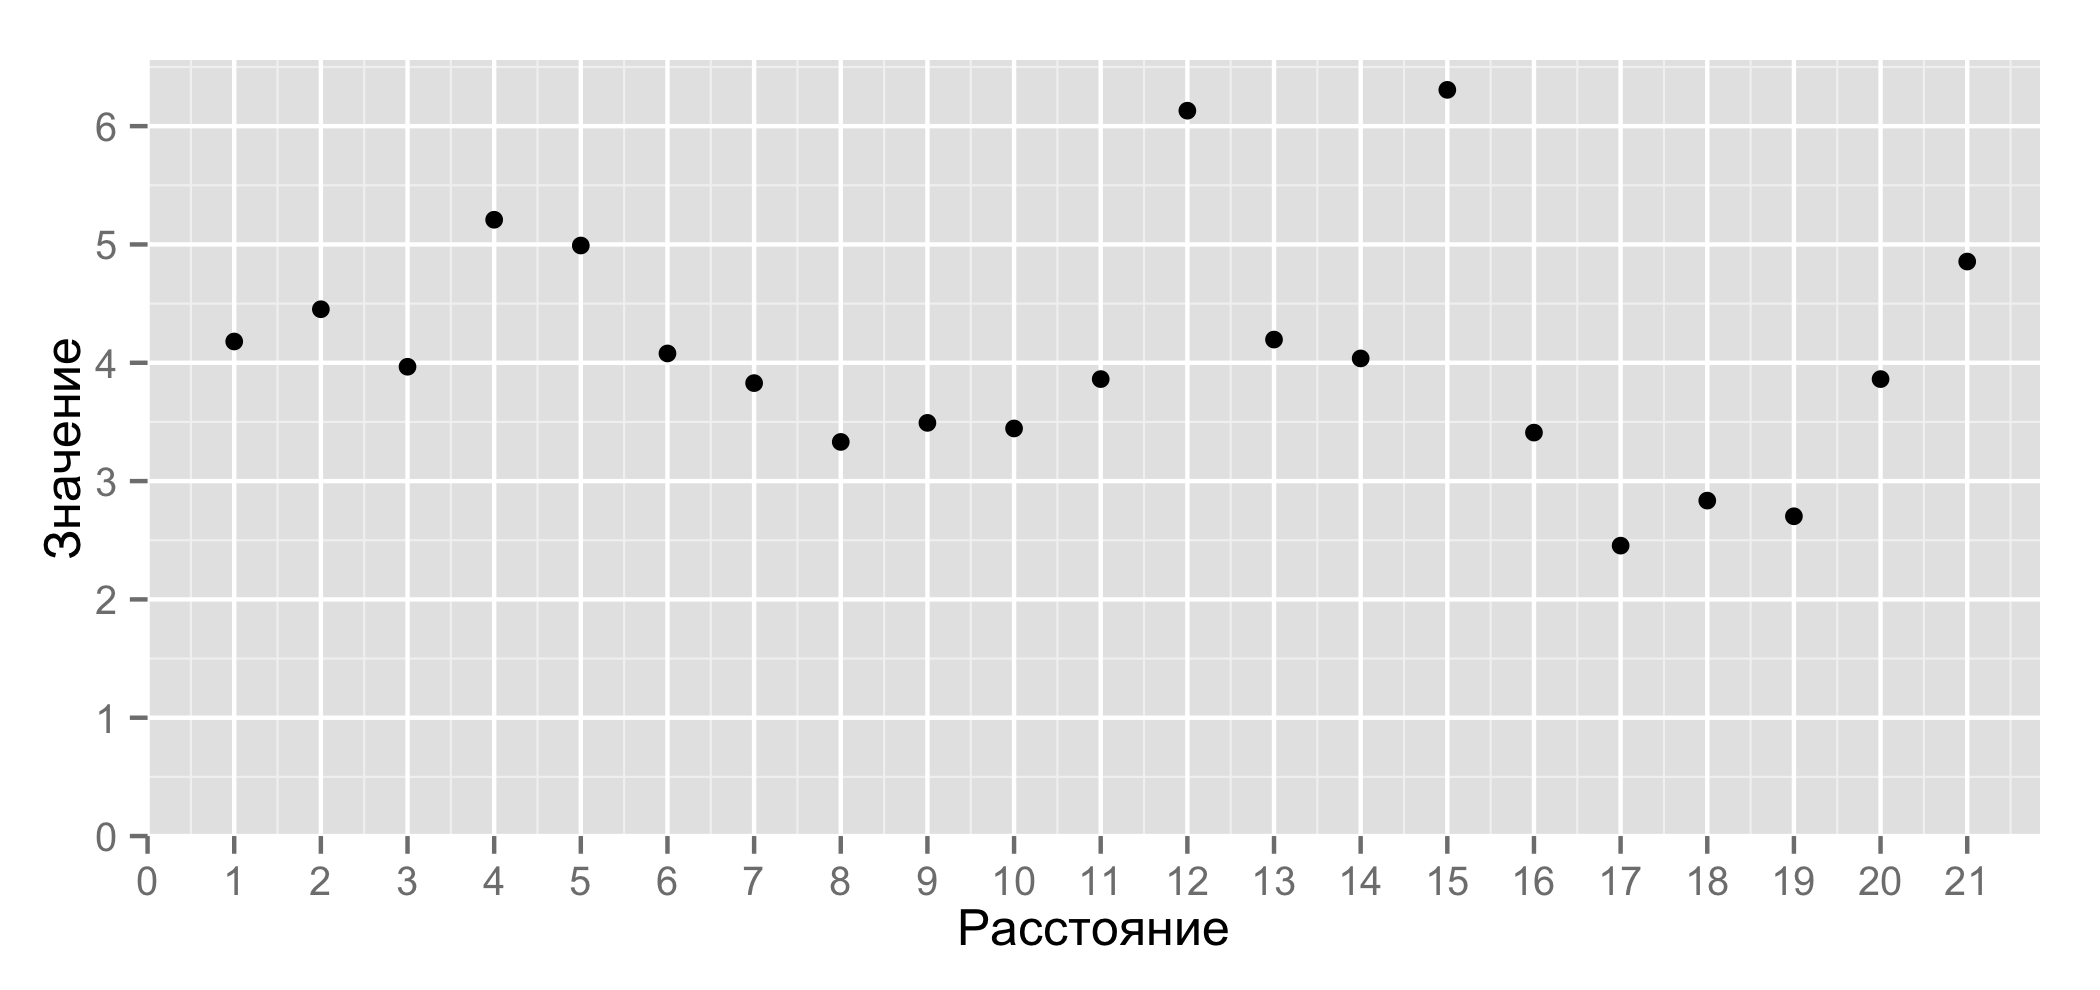
\includegraphics[width=4.5in]{../../figures/variogram/lin-variogram.png}
  \end{columns}
\end{frame}

\begin{frame}
  \frametitle{Линейная модель с порогом}   % Insert frame title between curly braces
  \begin{columns}[c]
  \column{2in}  % slides are 3in high by 5in wide
  Подобранная модель: $ 0.3 + 4 \cdot Lin(h, 6.2) $
  \column{3in}
   \framebox{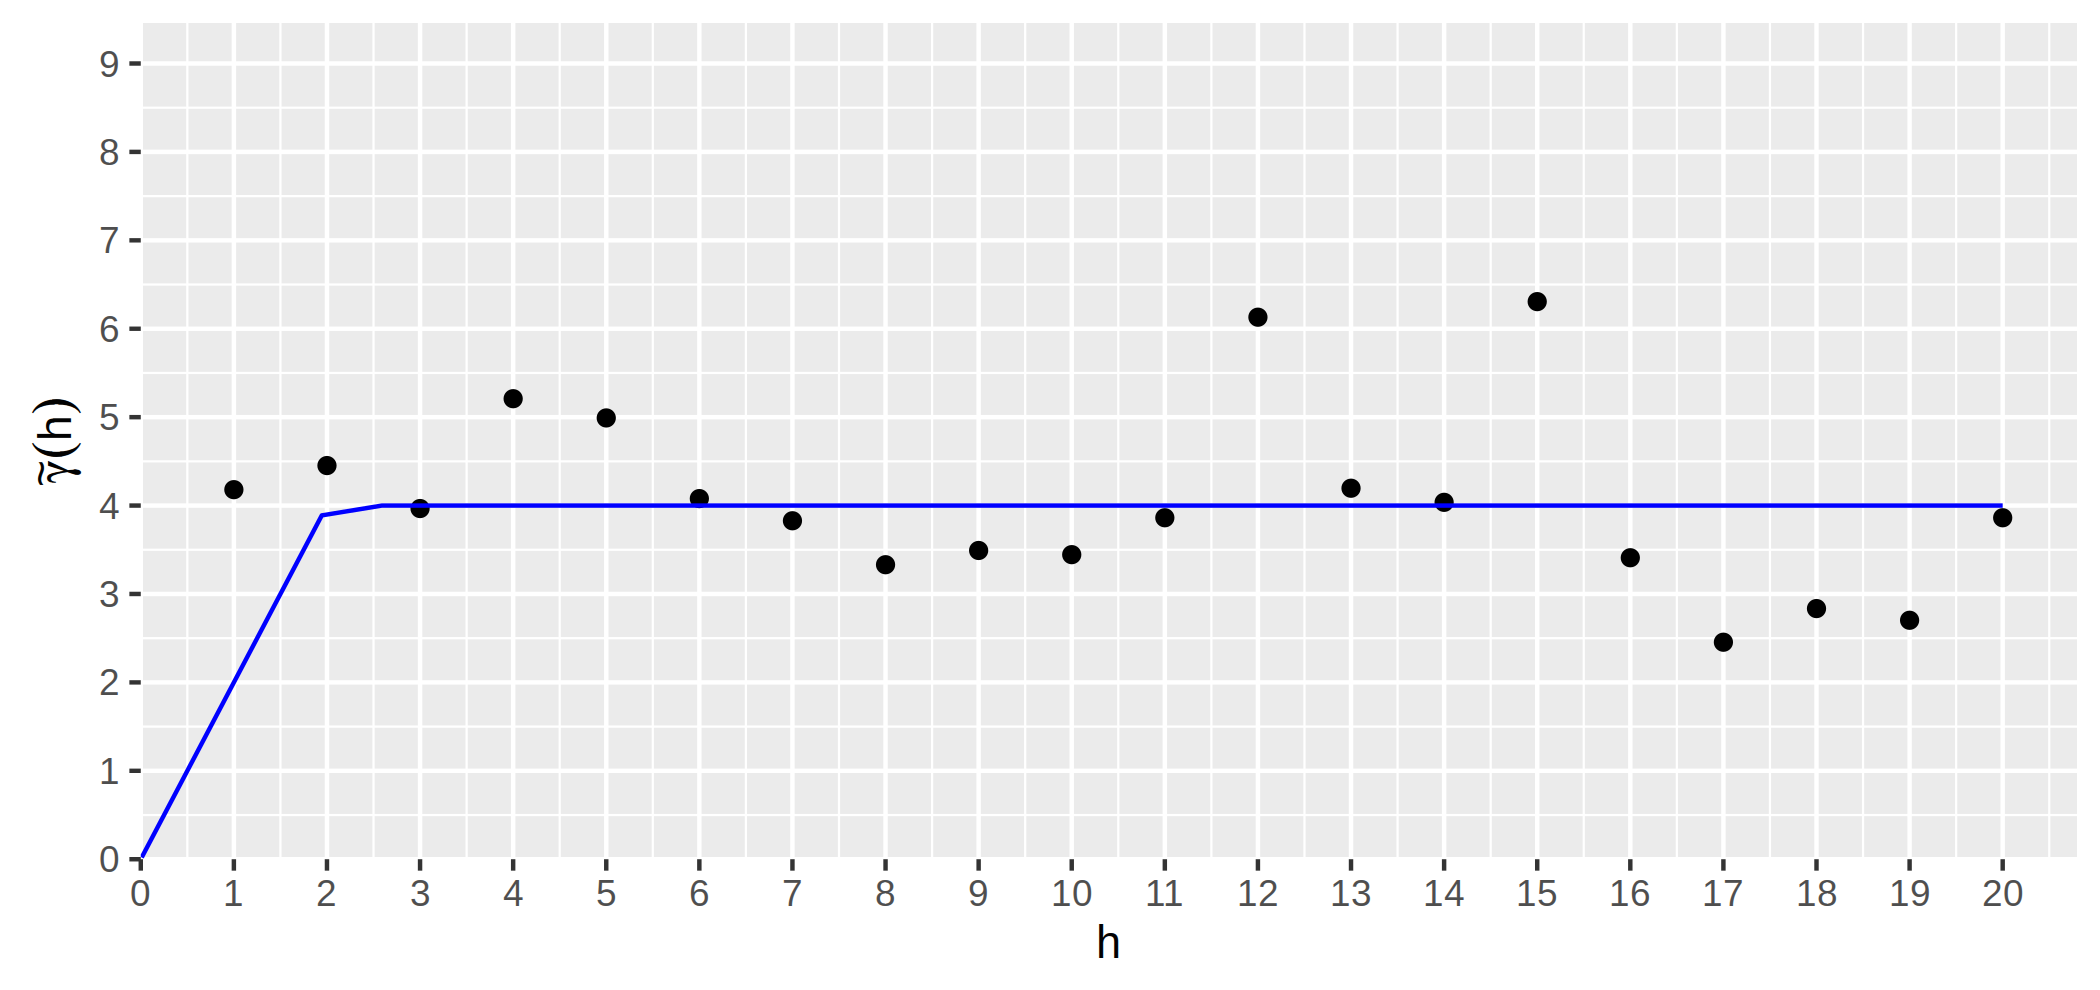
\includegraphics[width=3in]{../../figures/variogram/lin-fit-adapt-modeled.png}}
  \end{columns}
\end{frame}

\subsection{Кригинг}
\begin{frame}
  \frametitle{Прогнозирование методом ординарного кригинга}   % Insert frame title between curly braces
   \begin{columns}[c]
   \column{4.5in}
   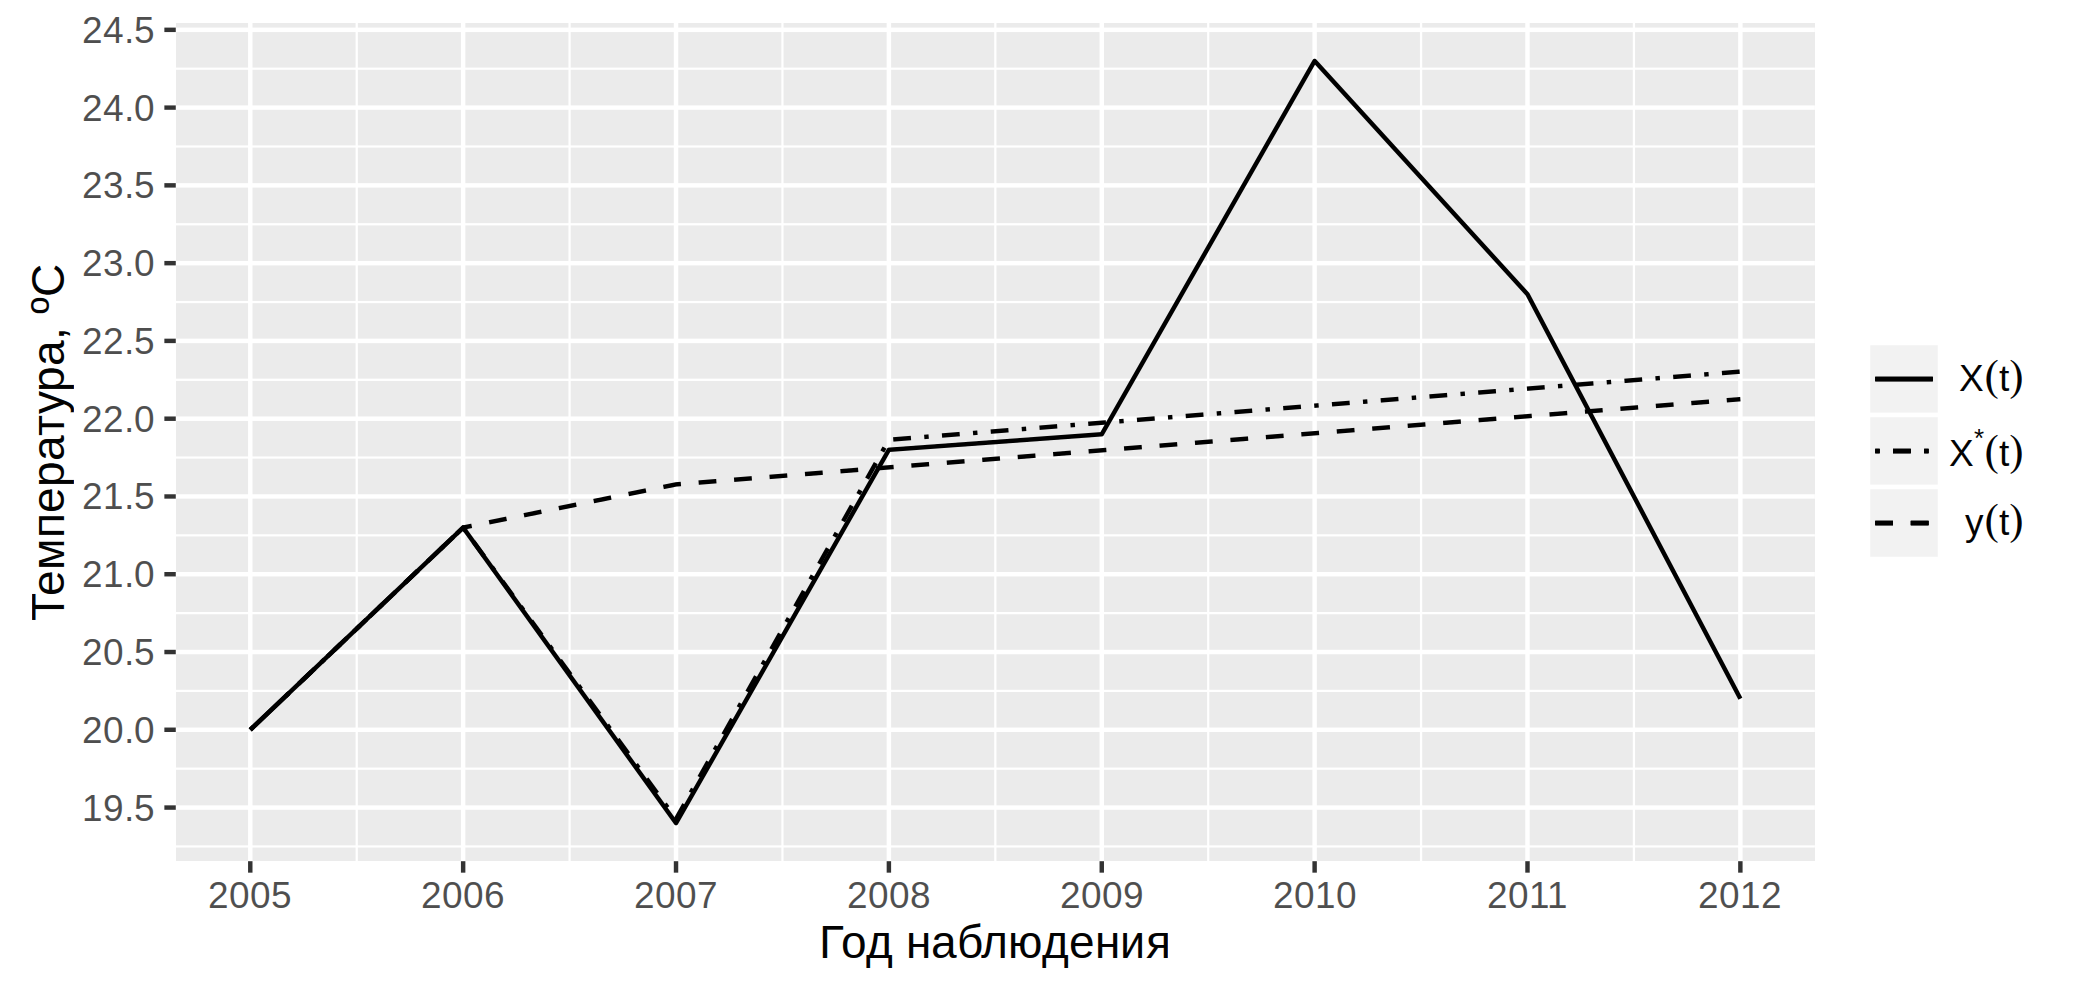
\includegraphics[width=4.5in]{../../figures/variogram/lin-fit-adapt-cross-prediction.png}
  \end{columns}
\end{frame}

\begin{frame}
  \frametitle{Периодическая модель}   % Insert frame title between curly braces
  \begin{columns}[c]
  \column{2in}  % slides are 3in high by 5in wide
  Подобранная модель: $ 4 \cdot Per(h, 0.898) $
  \column{3in}
   \framebox{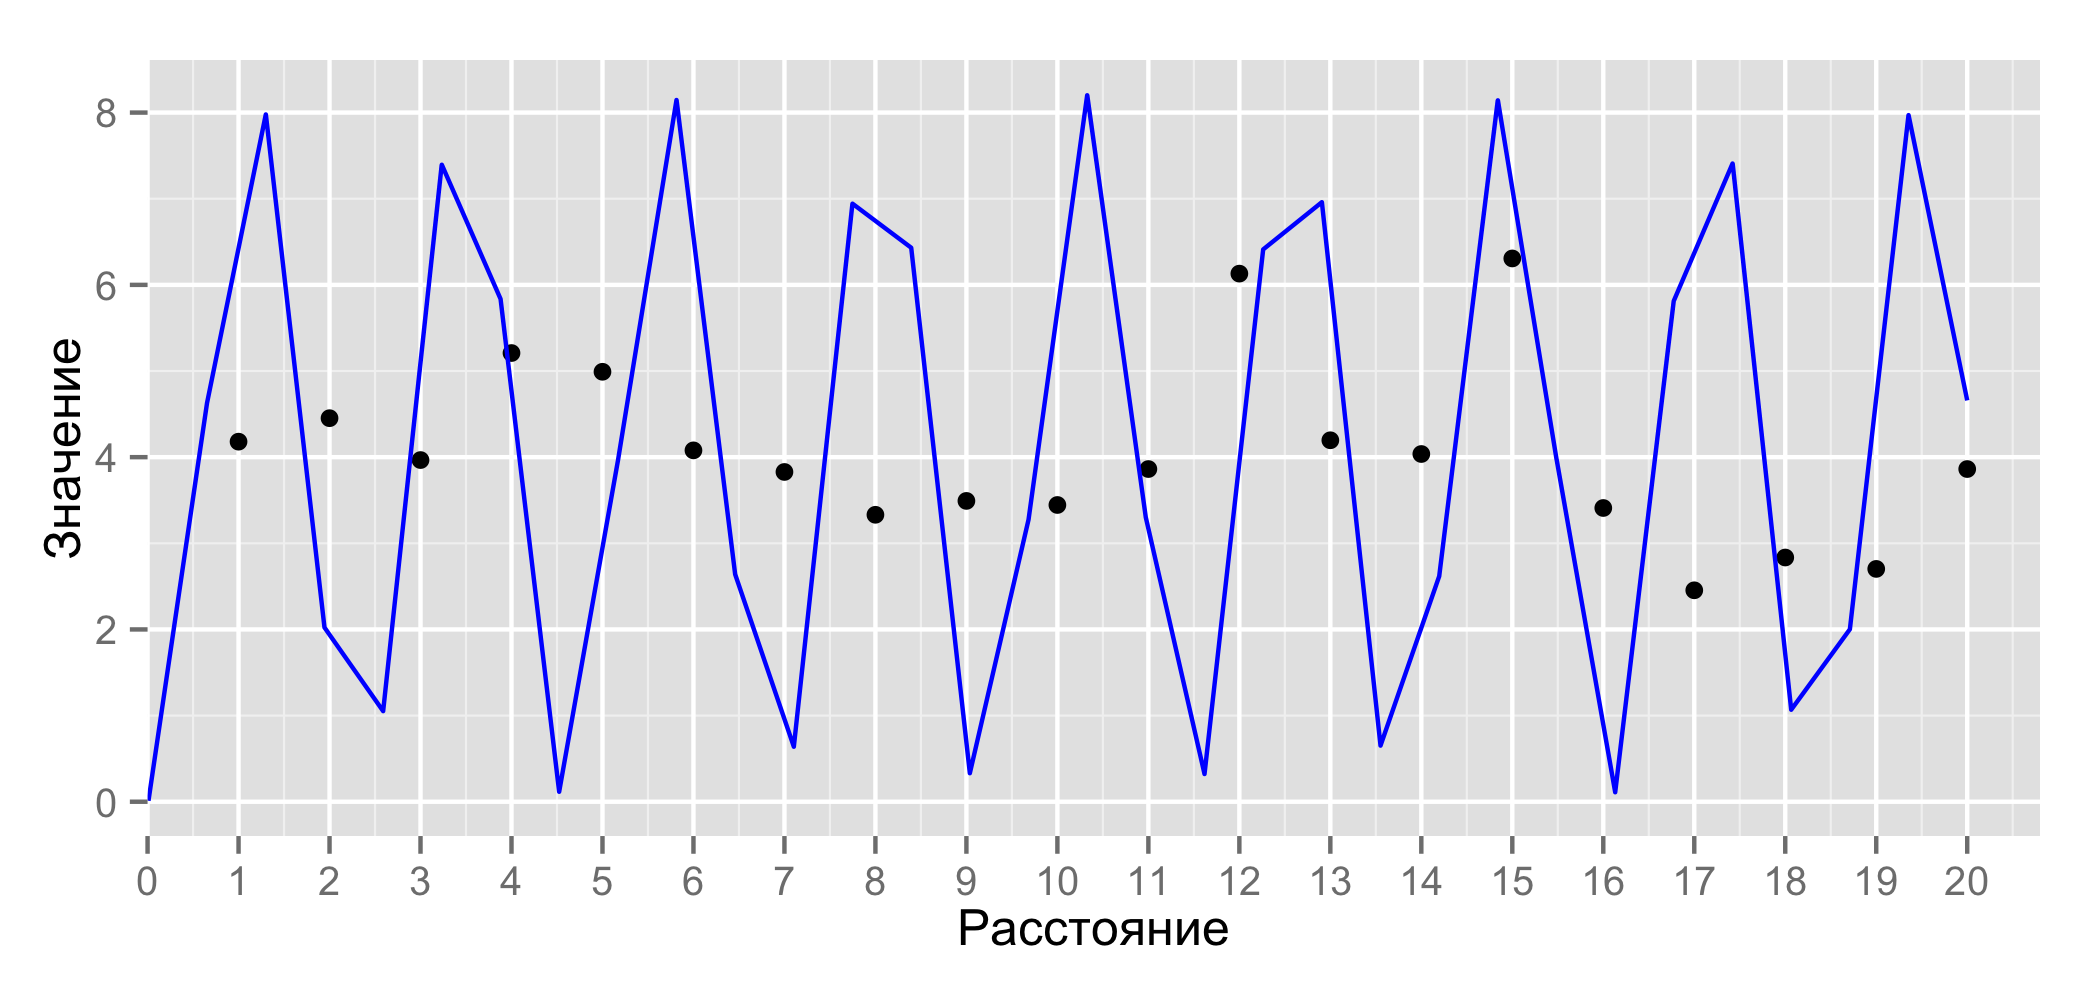
\includegraphics[width=3in]{../../figures/variogram/per-fit-cv-modeled.png}}
  \end{columns}
\end{frame}

\begin{frame}
  \frametitle{Прогнозирование методом ординарного кригинга}   % Insert frame title between curly braces
   \begin{columns}[c]
   \column{4.5in}
   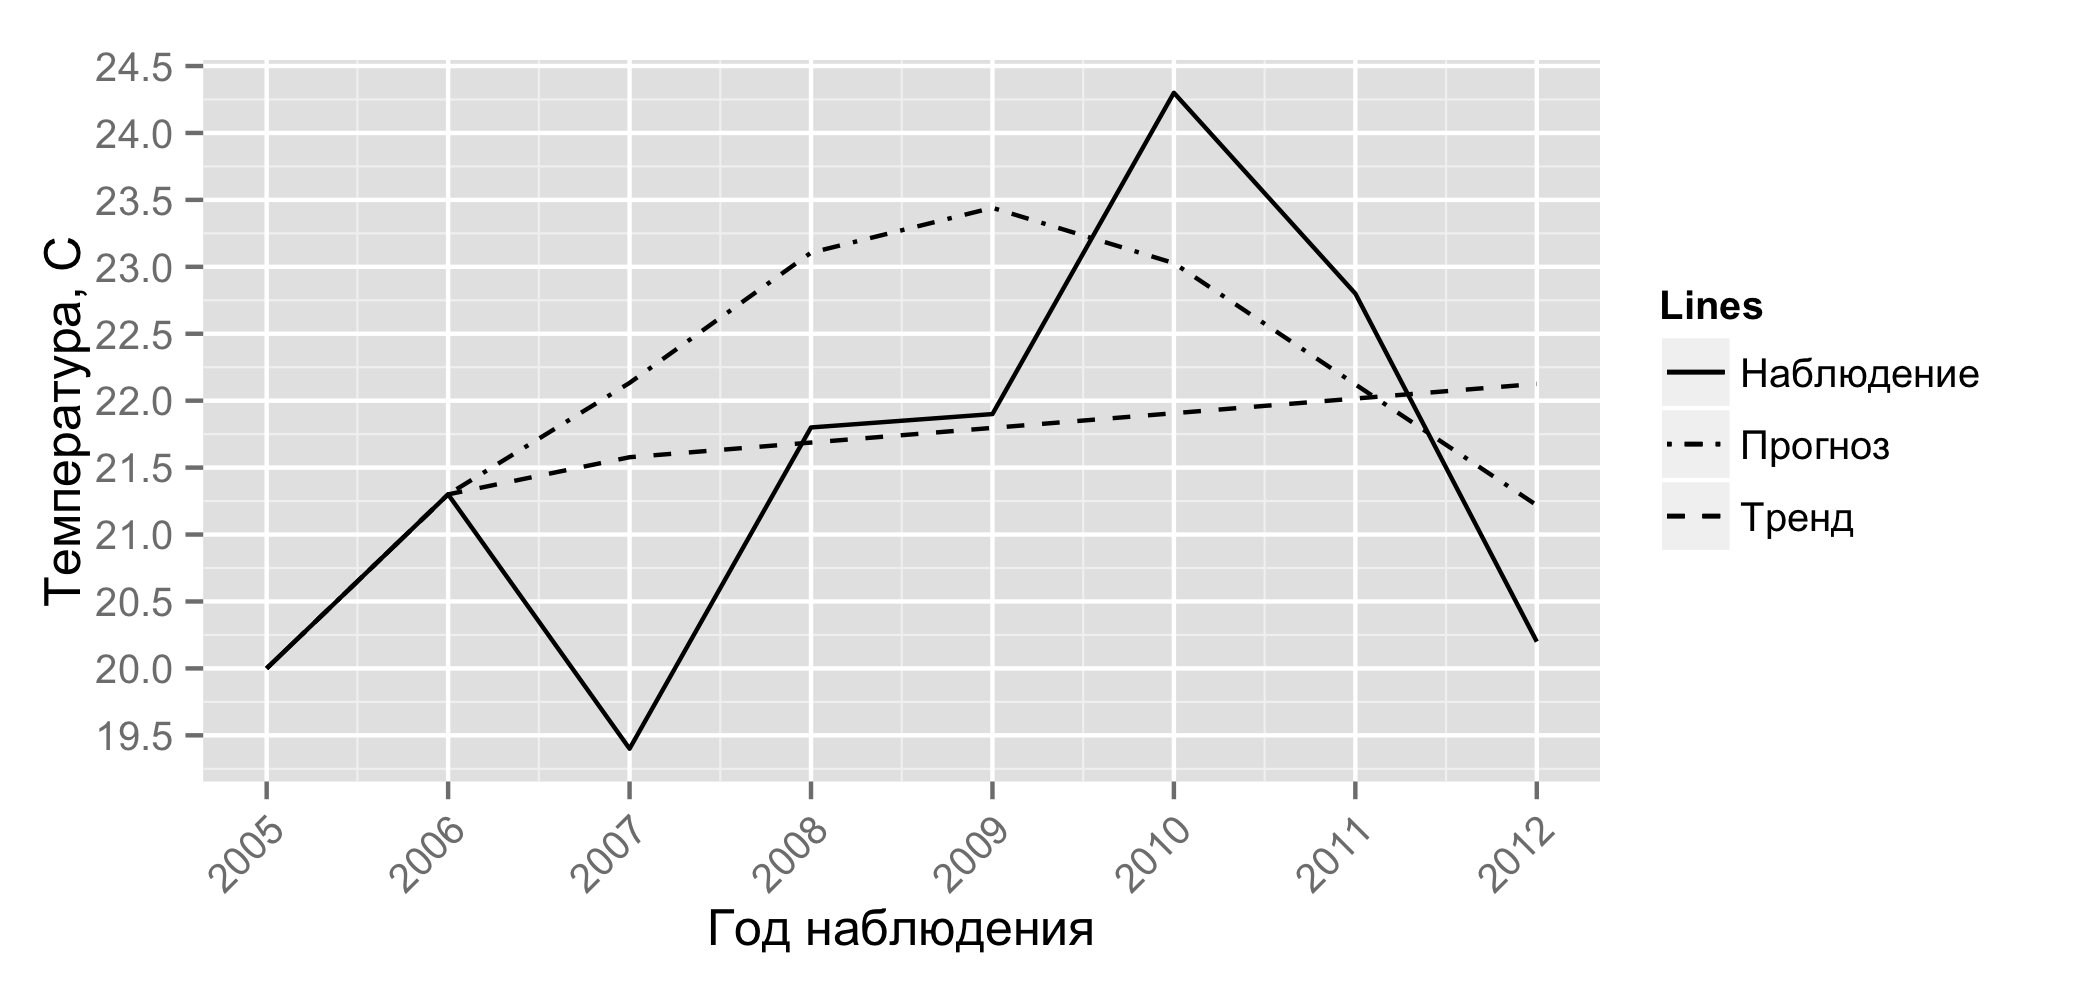
\includegraphics[width=4.5in]{../../figures/variogram/per-fit-cv-cross-prediction.png}
  \end{columns}
\end{frame}

\subsection{Автоматический подбор}

\begin{frame}
  \frametitle{Периодическая модель}   % Insert frame title between curly braces
  \begin{columns}[c]
  \column{2in}  % slides are 3in high by 5in wide
  Подобранная модель: $ 3.8 + 0.32 \cdot Per(h, 1.3) $
  \column{3in}
   \framebox{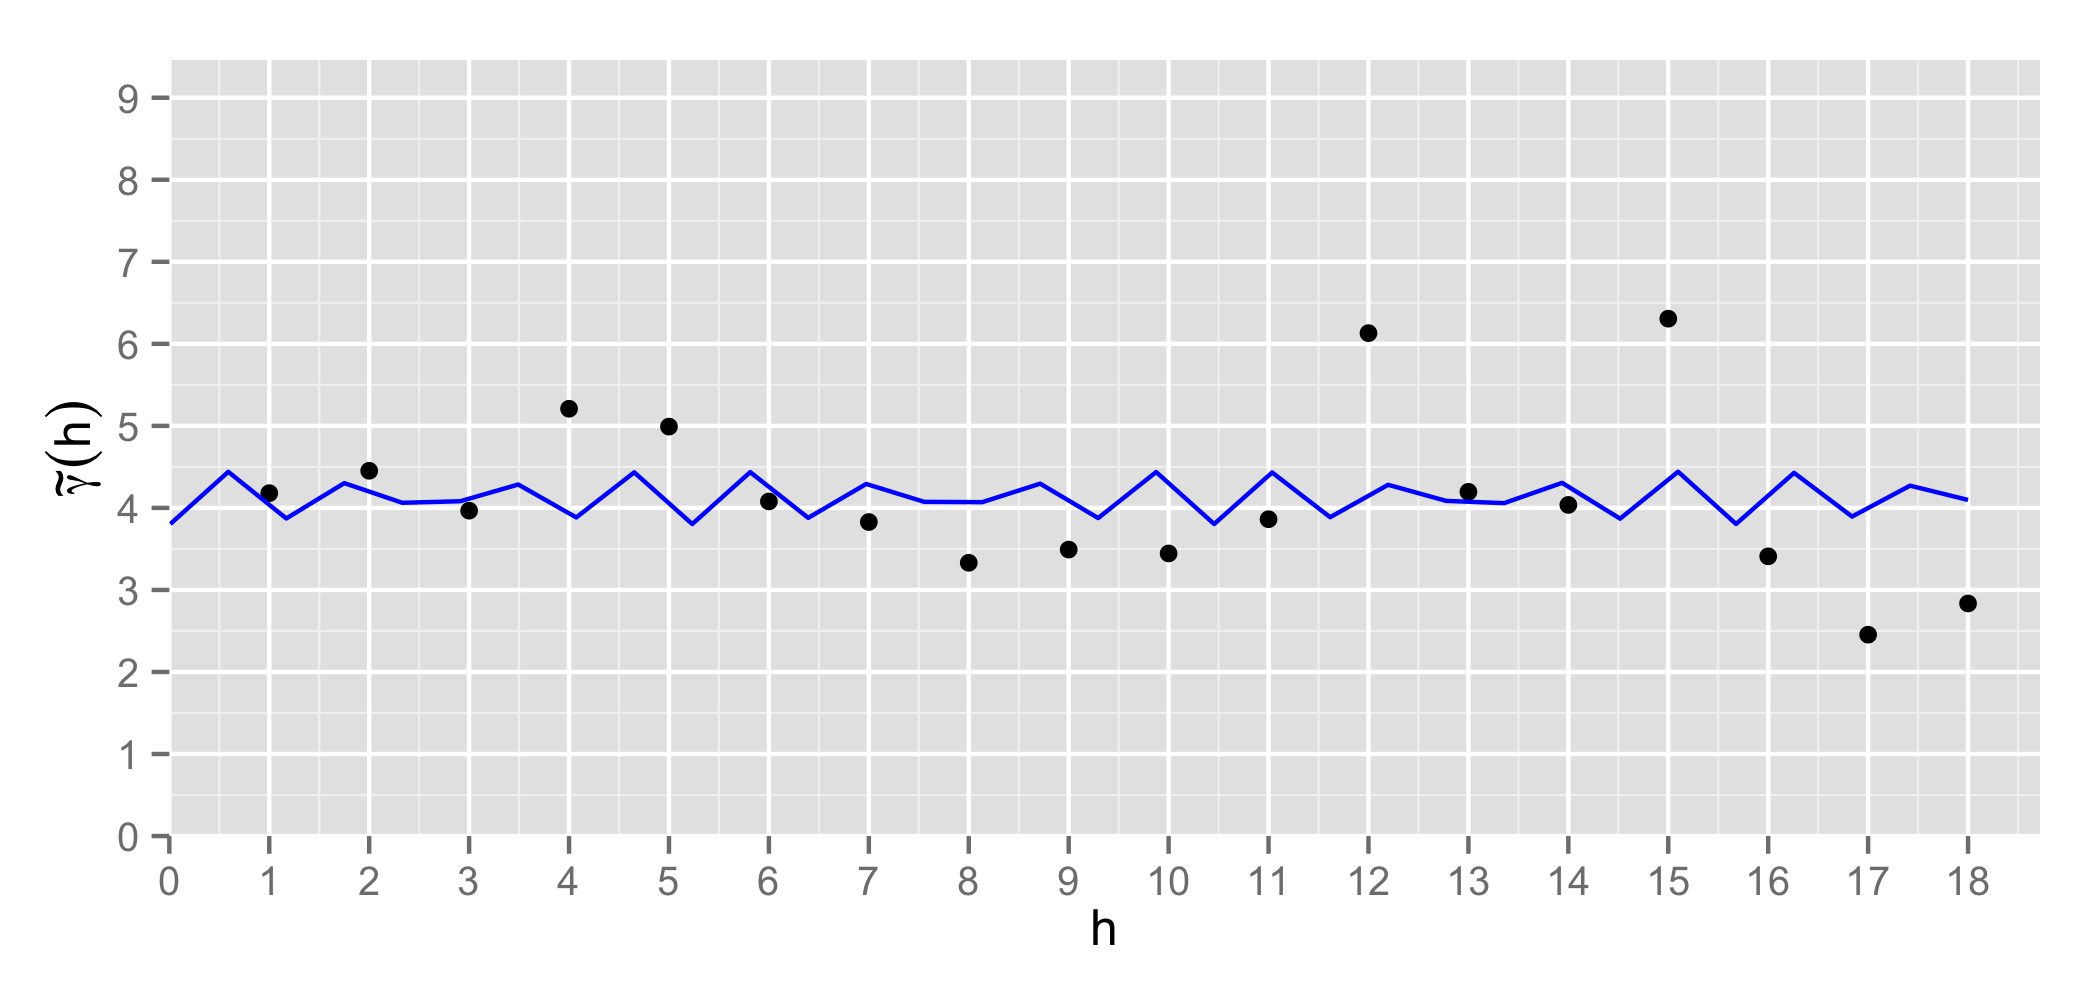
\includegraphics[width=3in]{../../figures/variogram/auto-class-18-modeled.png}}
  \end{columns}
\end{frame}

\begin{frame}
  \frametitle{Прогнозирование методом ординарного кригинга}   % Insert frame title between curly braces
   \begin{columns}[c]
   \column{4.5in}
   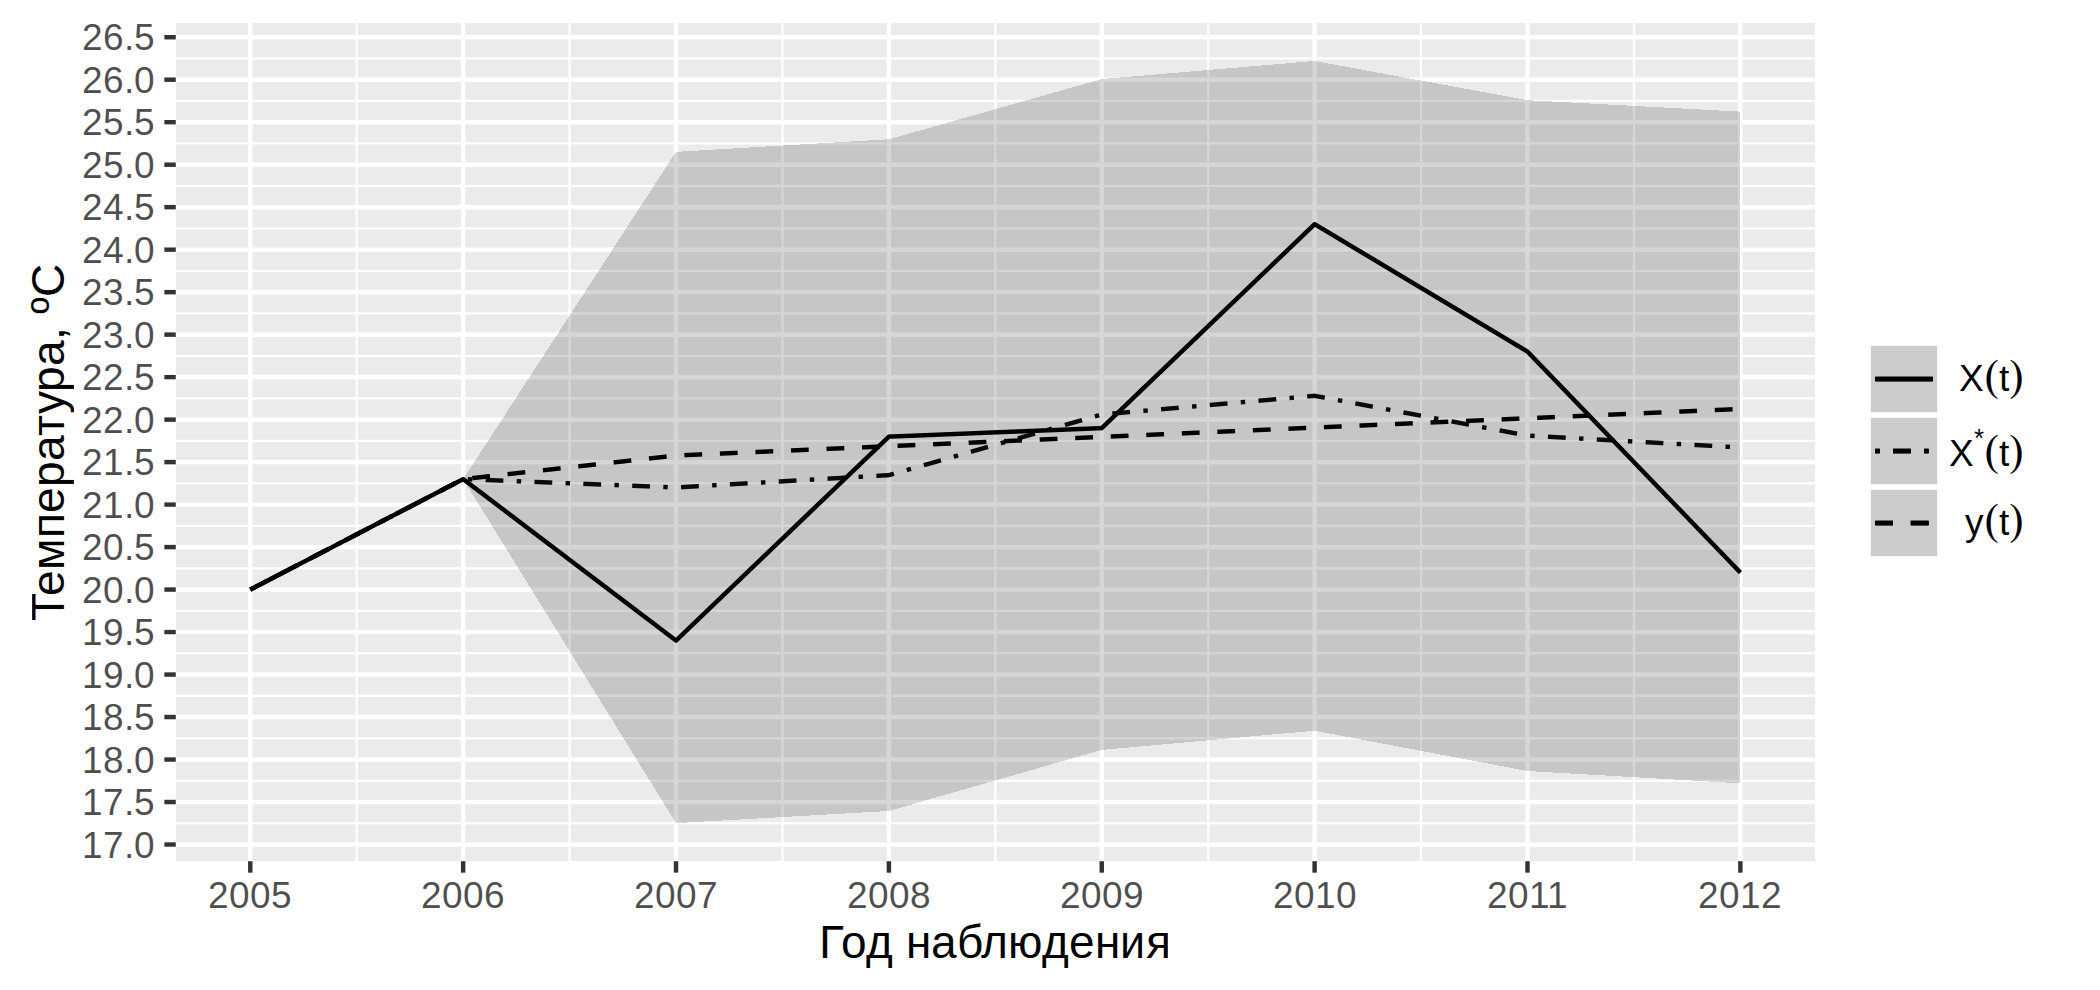
\includegraphics[width=4.5in]{../../figures/variogram/auto-class-18-cross-prediction.png}
  \end{columns}
\end{frame}

\begin{frame}
  \frametitle{Волновая модель}   % Insert frame title between curly braces
  \begin{columns}[c]
  \column{2in}  % slides are 3in high by 5in wide
  Подобранная модель: $ 4.11 + 1.65 \cdot Wav(h, 3.59) $
  \column{3in}
   \framebox{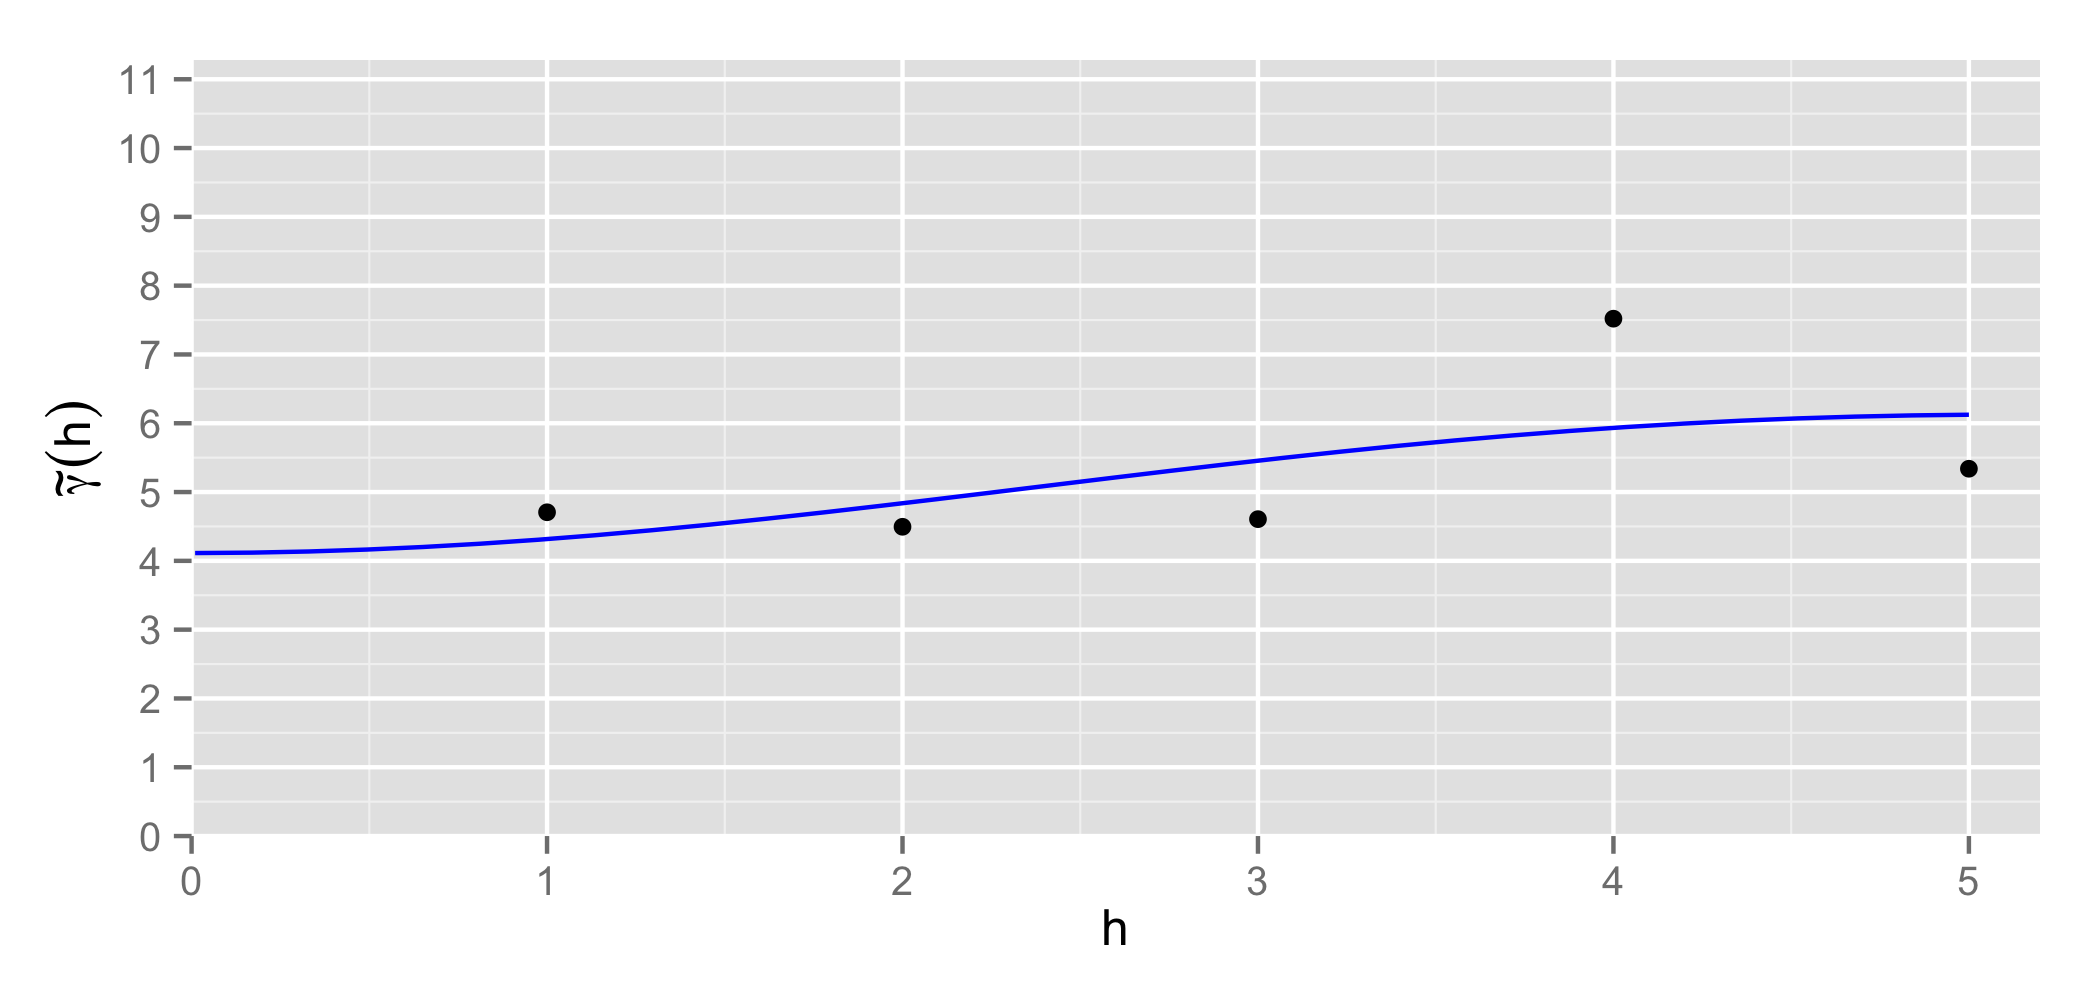
\includegraphics[width=3in]{../../figures/variogram/auto-rob-5-modeled.png}}
  \end{columns}
\end{frame}

\begin{frame}
  \frametitle{Прогнозирование методом ординарного кригинга}   % Insert frame title between curly braces
   \begin{columns}[c]
   \column{4.5in}
   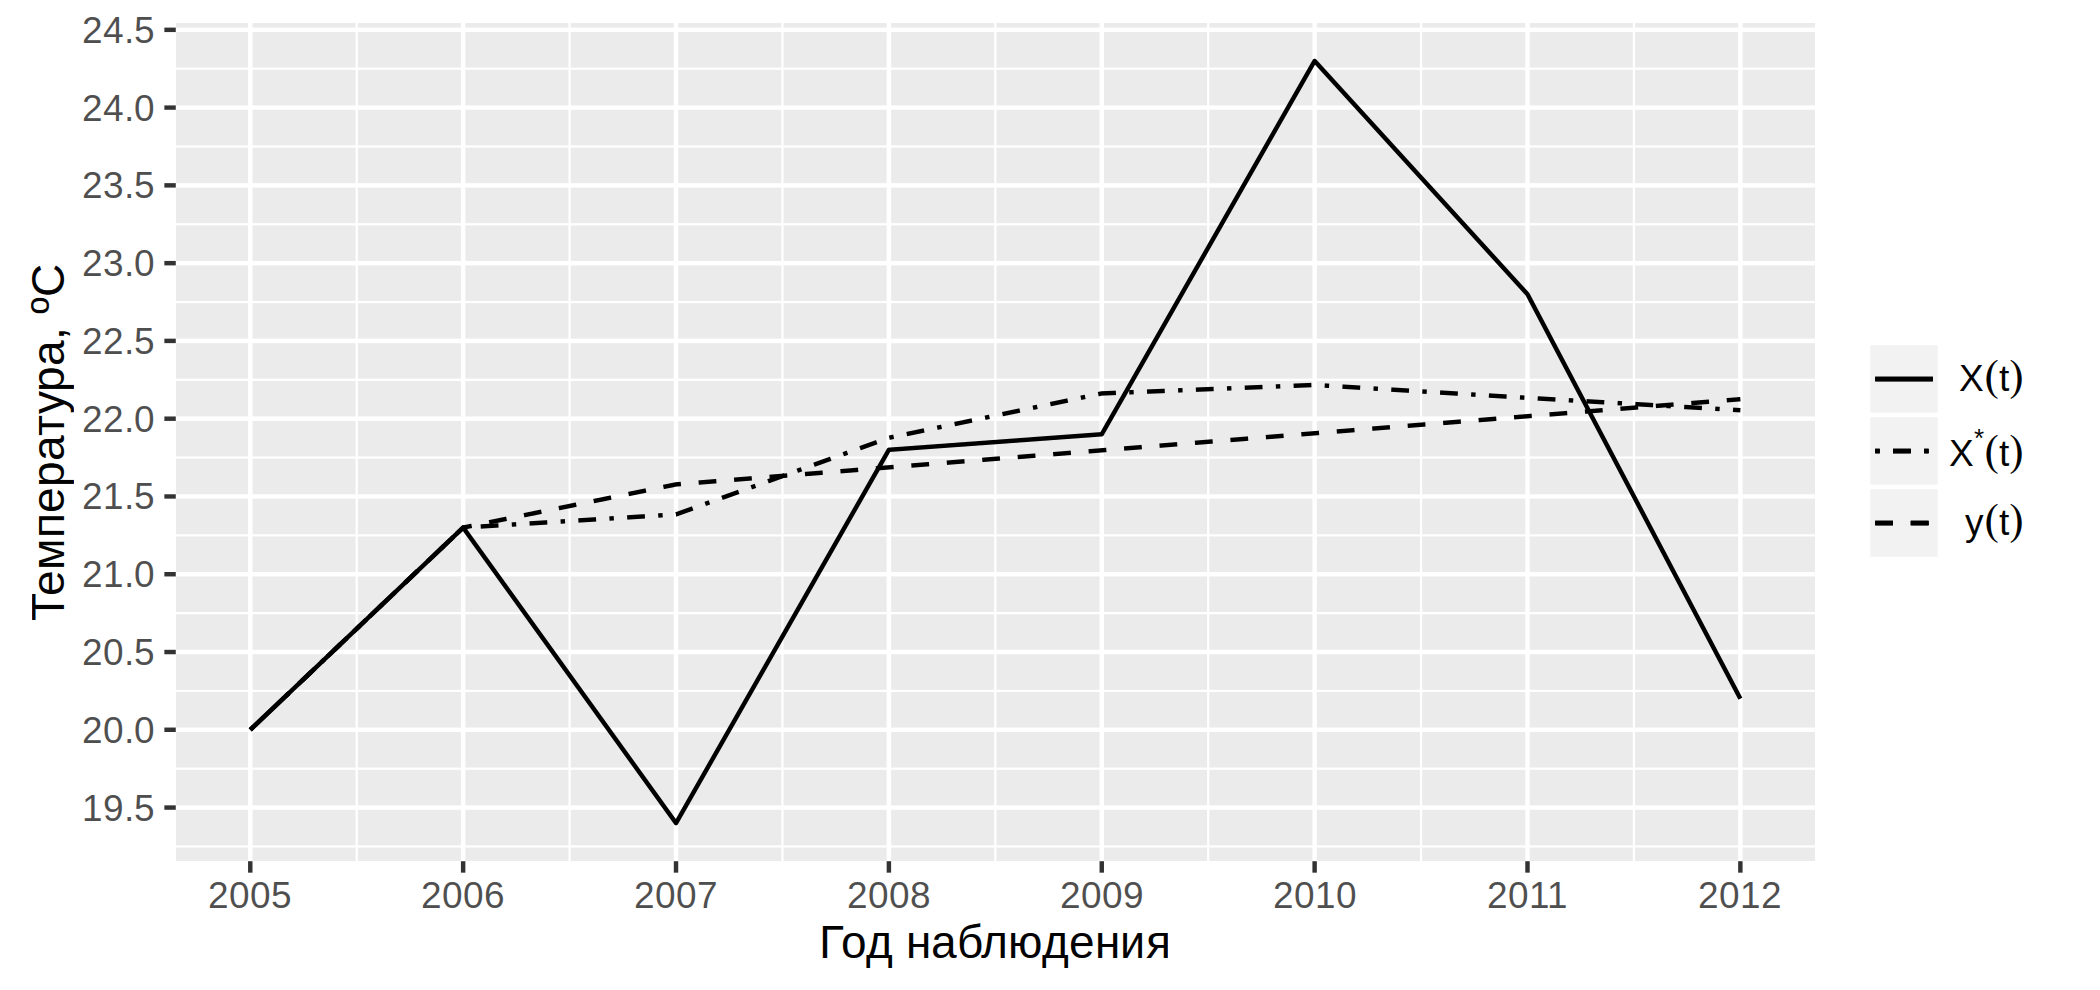
\includegraphics[width=4.5in]{../../figures/variogram/auto-rob-5-cross-prediction.png}
  \end{columns}
\end{frame}

% \subsection{}
% \begin{frame}
%   \frametitle{}   % Insert frame title between curly braces
%    \begin{columns}[c]
%    \column{1.3in}
%   Спасибо за внимание
%   \end{columns}
% \end{frame}
\end{document}